\chapter{State of Art}%
\label{chapter:stateofart}

%  mantain this? 
% \begin{introduction}
% In this chapter, the evolution leading to Industry 5.0 contextualizes the importance of technological advancements. 
% The focus is on Industry 5.0, particularly its transition from autonomous robots to the emerging dynamics of \ac{HRC}.
% The critical need for collaborative scenarios between humans and robots is highlighted, emphasizing the transformative potential of such partnerships. 
% Moreover, the integration of digital realities with \ac{DT} in Industry 5.0 is evaluated for its impact on enhancing \ac{HRI}, signaling a new era of efficiency and 
% collaboration in industrial operations.
% \end{introduction}


\section{Key Drivers of Industry 5.0}
\label{section:industry-evolution}
With the advent of Industry 4.0 and the emerging concept of Industry 5.0, the industry environment has witnessed significant transformations. Understanding this progress is crucial to contextualize the technological advancements and the shift towards more human-centric manufacturing processes.

\subsection{Industry 4.0: The Fourth Industrial Revolution}

Industry 4.0 represents the integration of cutting-edge digital technologies into manufacturing processes, leading to the emergence of smart factories. It leverages advanced systems such as \ac{CPSS}, the \ac{IOT}, robotics, Augmented Reality \ac{AR}, simulation, cloud computing, and big data analytics, as illustrated in Figure~\ref{fig:key-tech-industry-4}. This paradigm signifies a fundamental shift towards interconnected, intelligent, and digitally-driven manufacturing ecosystems, revolutionizing the way products are conceived, manufactured, and delivered, while enhancing production efficiency, flexibility, and innovation~\cite{Moller2022, Ahmed2022}.

\begin{figure}[!htbp]
    \centering
    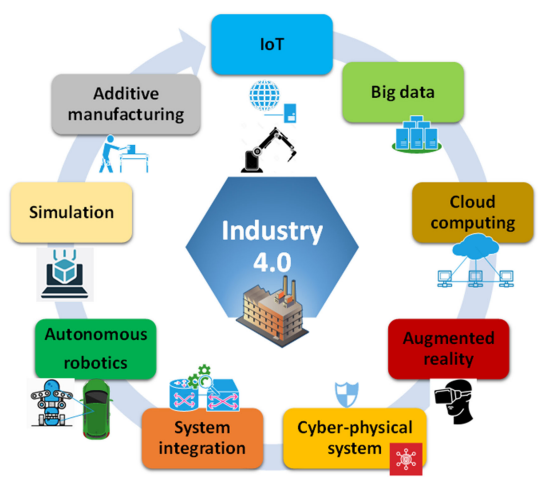
\includegraphics[width=0.6\linewidth]{figs/key-tech-industry-4.png}
    \caption{Key enabling technologies in Industry 4.0~\cite{Ahmed2022}}
    \label{fig:key-tech-industry-4}
\end{figure}

With advancements in \ac{AI}, industrial processes can achieve unprecedented performance levels, often exceeding human capabilities. These \ac{AI}-driven systems enable robots to perform tasks that may be too hazardous, complex, or delicate for humans, such as handling dangerous materials or managing microscopic elements. Despite this extraordinary potential, it is important to recognize that current industrial robots are not as "smart" as humans in many contexts and, even though these robots are capable of performing highly skilled tasks, they frequently operate under strict, pre-programmed limits~\cite{Ahmed2022}.

Although Industry 4.0 has undoubtedly increased productivity, flexibility, and automation in industrial environments, it has also led to concerns regarding the diminishing role of human operators. This relentless push towards full automation has, in some cases, reduced human involvement in critical decision-making processes, leading to a more machine-centric production landscape~\cite{GOLOVIANKO2023102}.

\subsection{Industry 5.0: Reintegrating the Human Element}

Approximately a decade after the launch of Industry 4.0, the European Commission introduced the Industry 5.0 concept in response to new societal challenges~\cite{industry5}. The growing concerns about the exclusion of human operators in Industry 4.0 systems, coupled with the limitations of full automation, paved the way for this new industrial paradigm. Industry 5.0 seeks to reintroduce the human element into industrial ecosystems, emphasizing greater human involvement in manufacturing processes~\cite{su11164371}.

The main goal consists on combining the strengths of humans and machines to achieve more sustainable, efficient, and human-centered production systems. This shift reflects the realization that, while machines excel at repetitive, dangerous, or complex tasks, humans provide irreplaceable creativity, adaptability, and problem-solving abilities~\cite{10577684}. Industry 5.0 aims to strike a balance between technological advancement and human-centric values, fostering environments where humans work alongside advanced technologies to achieve greater societal and environmental outcomes~\cite{GOLOVIANKO2023102}.


% While Industry 4.0 focused on pushing the limits of automation and data-driven production, Industry 5.0 reintroduces the importance of human collaboration. 
Recognizing that humans and machines each have unique advantages that can complement each other, the key technological drivers of Industry 5.0 build upon the advancements of Industry 4.0 in order to address their limitations.

\begin{itemize}
    \item \textbf{Artificial Intelligence and Cognitive Computing:} These technologies continue to evolve, enabling robots and automation systems to work alongside humans in ways that enhance productivity without fully replacing them. \ac{AI} allows for more intuitive \ac{HMI}, where machines can understand and respond to human needs more effectively.

    \item \textbf{Collaborative Robots (Cobots):} are engineered to ensure safe, collaborative operation alongside human workers, facilitating not only intuitive interactions but also fostering efforts that leverage the unique strengths of both humans and robots. Their integration is driven by the need to create systems that enable seamless, user-friendly human-robot collaboration, in full alignment with the guiding principles of Industry 5.0. This paradigm shift redefines traditional employment roles by emphasizing human-robot interaction, with a focus on communication and coordination with robotic systems and advanced \ac{AI}~\cite{10577684}.

    \item \textbf{Digital Twins (\ac{DT}):} represent a pivotal technological advancement in Industry 5.0. They provide visual models that enhance comprehension and facilitate the evaluation of goods, processes, and production systems. By allowing real-time monitoring and simulation, \ac{DT} help optimize manufacturing processes, bridging the gap between the virtual and physical worlds~\cite{10577684}.

    \item \textbf{Human-Centric Automation:} Emphasis is placed on using technology to augment human capabilities rather than replace them, fostering a more inclusive, creative, and flexible manufacturing environment. This approach ensures that technology empowers human workers, enabling them to focus on tasks requiring intuition and creativity.

    \item \textbf{Advanced Human-Machine Interfaces:} The development of intuitive interfaces, by integrating technologies such as \ac{AR} and \ac{VR}, facilitates better communication between humans and machines. These interfaces allow for more natural interactions, improving understanding and efficiency in collaborative tasks.

    \item \textbf{Sustainable and Resilient Manufacturing:} Industry 5.0 also focuses on sustainability and resilience, integrating environmental considerations into manufacturing processes. This includes optimizing resource usage and reducing waste, aligning technological advancement with ecological responsibility.
\end{itemize}

By integrating these key drivers, Industry 5.0 addresses the challenges identified in Industry 4.0, promoting harmonious collaboration between humans and machines. This synergy aims to enhance productivity while preserving the unique contributions of human workers, ultimately leading to more innovative, sustainable, and human-centered industrial practices.


% %%%%%%%%%%%%%%%%%%%%%%%%%%%%%%%%%%%%%%%%%%%%%%%%%%%%%%%%%%%%%%%%

% \section{Introduction to Industry 5.0} As a response to the increasing automation and the need for greater human involvement in manufacturing 
% processes, "Industry 5.0" seeks to reintroduce the human element into industrial ecosystems. Unlike Industry 4.0, which prioritized automation and 
% machine autonomy, Industry 5.0 emphasizes human-robot collaboration, where the strengths of humans and machines are combined to achieve more sustainable, 
% efficient, and human-centered production systems. This shift reflects the realization that while machines excel at repetitive, dangerous, or complex tasks,
% humans provide irreplaceable creativity, adaptability, and problem-solving abilities.

% Industry 5.0 seeks to strike a balance between technological advancement and human-centric values, fostering environments where humans work alongside 
% advanced technologies to achieve greater societal and environmental outcomes \cite{GOLOVIANKO2023102}.

\section{Human-Robot Collaboration}
%%%% estender um pouco mais e fazer ponte para collaboration scenarios / digital realities
\label{subsection:human-robot-collab}
% \input{chapters/stateofart/subsections/human-robot-collab}

Human-Robot Interaction (\ac{HRI}) is an extensive field dedicated to examining the interactions and coexistence of humans and robots in shared spaces, whose objective consists on enhancing these interactions by designing robots that are safe, effective and compatible for assisting and cooperating with humans in diverse roles, rather than replacing them \cite{Ogenyi2021}.
This involves developing robots that are, not only autonomous, but also capable of understanding and communicating with humans, as well as predicting
human-behavior and learning from human feedback. 

However, \ac{HRI} can be broken down into different forms of interaction, whose categorization is based on various factors that define how 
humans and robots share the workspace. This disctinction is represented in the figure \ref{fig:collab} and can be summarized as follows \cite{Jahanmahin2022}:

\begin{figure}[!htbp]
    \centering
    % \hspace{-1.3cm}
    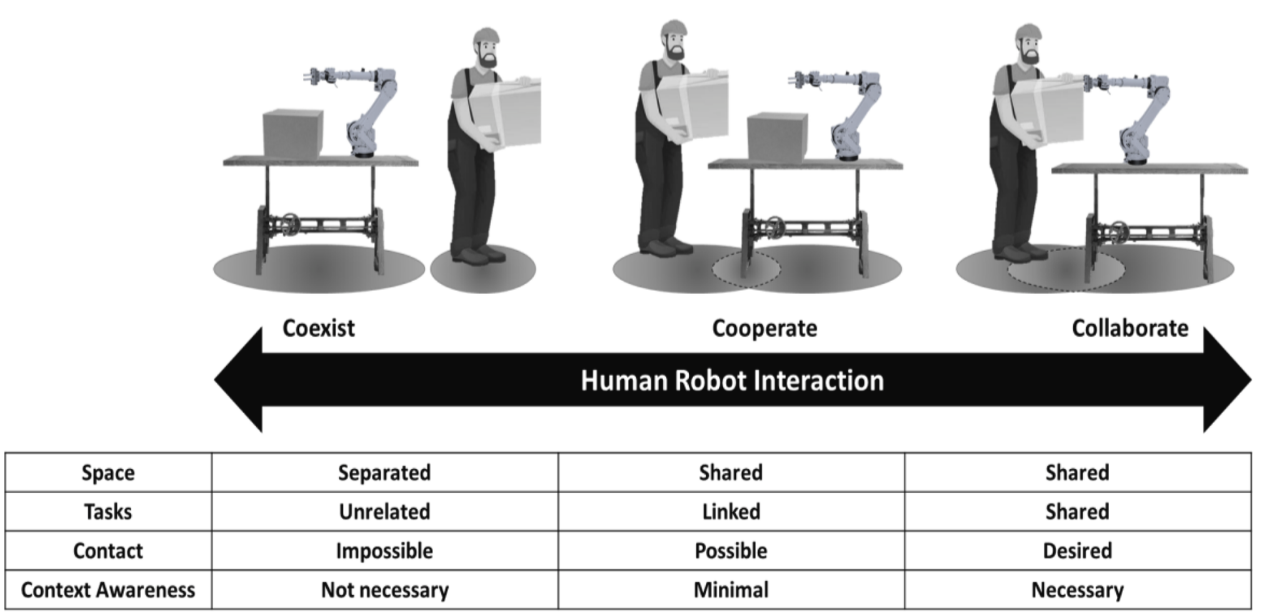
\includegraphics[width=1.0\linewidth]{figs/collab-coex-coopr.png}
    \caption{Different levels of \ac{HRI} - \cite{Jahanmahin2022}} 
    \label{fig:collab}
\end{figure} 

\begin{itemize}
    \item \textbf{\ac{HRCx}}: In this form of interaction, humans and robots do not directly interact.
    Both carry out their tasks independently, avoiding contact. Usually this interaction does not involve synchronized work 
    or communication between the two parties.

    \item \textbf{\ac{HRCp}}: Here, humans and robots share both the workspace and the task objective. Cooperation occurs when humans
    and robots work towards a common goal, and advanced technologies such as sensors or machine vision rarely may be used to detect and prevent collisions.
    However, there is limited physical interaction between them.

    \item \textbf{Human-Robot Collaboration (\ac{HRC})}: This is the most integrated form of \ac{HRI}, where humans and robots, not only share the workspace and objectives, but also interact directly.
    %  as shown in the picture \ref{fig:hrc-workstation}. 
    
    % One key area within Human-Robot Interaction (\ac{HRI}) is Human-Robot Collaboration (\ac{HRC}), which specifically focuses on scenarios where humans and robots cooperate directly to achieve common goals.

    In \ac{HRC}, physical contact may occur (e.g., through shared manipulation of an object) or there can be non-physical collaboration, such as verbal communication, gestures, or pattern recognition. In collaborative environments, humans usually perform tasks requiring fine motor skills or decision-making, while robots handle repetitive, strenuous, or hazardous tasks.

\end{itemize}

% explanation of the below figure
Below, the figure \ref{fig:hrc-workstation} illustrates a \ac{HRC} workspace, showcasing the interaction between a human worker and a robot within a shared environment. The workspace is divided into distinct yet overlapping areas: the robot's work envelope and the human's work envelope. These areas reflect the respective tasks of each party, with the robot likely performing repetitive or automated tasks, such as material handling within the feeding system, while the human focuses on more intricate tasks requiring dexterity and decision-making.

The overlapping shared workspace demonstrates the core principle of \ac{HRC}, where humans and robots work together toward common goals, necessitating real-time coordination and communication. In this setup, advanced sensing technologies or machine vision are essential to ensure safety and prevent collisions, allowing both the human and robot to operate efficiently within close proximity.

This image underscores how robots, rather than replacing humans, complement human skills by taking on routine, physically demanding tasks, while humans contribute with their cognitive abilities. This partnership reflects the broader vision of Industry 5.0, where human creativity and robotic precision are combined to create adaptable, human-centered industrial processes, enhancing both efficiency and safety in collaborative environments.

\begin{figure}[!htbp]
    \centering
    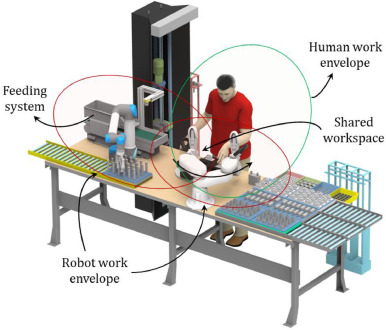
\includegraphics[width=0.55\linewidth]{figs/human-robot-collab-env.jpg}
    \caption{Human-robot collaborative workstation - \cite{MALIK2021102092}} 
    \label{fig:hrc-workstation}
\end{figure} 


These new robots featuring intelligent sensing and vision systems, envisioned to integrate the production line, are called "cobots". 
They represent the alternative to full automation, since industry specialists have stated it is not possible to completely remove the 
human within the manufacturing environment \cite{Weiss2021}.

%% adicionar figura correta e dar label - verificar depois esta questao do estado da arte aqui

%%%%%%%%%%%%%%%%%%%%%%%% analise do artigo sobre cobots - Human–Robot Collaboration in Manufacturing Applications: A Review - 2019
%%%%%%%%%%%%%%%%%%%%%%%% ver melhor esta parte abaixo, organizar melhor e adicionar referencias bem, imagens e o que está a faltar
\section{Collaborative Robots (Cobots)} 


In the past decade, the market has introduced a new category of robots known as collaborative robots, or "cobots." These are designed to interact 
physically with humans within the same workspace, devoid of the traditional barriers or protective cages typical in conventional robotic systems. 
Cobots are celebrated for their ability to quickly and inexpensively adapt layouts, although properly harnessing their potential requires a thorough 
understanding of their proper uses and characteristics, which can otherwise pose barriers to industry adoption \cite{robotics8040100}.


% \subsubsection{The Role and Benefits of Cobots}

Unlike traditional industrial robotic systems, which require extensive safety guarding and consequently reduce flexibility while increasing both costs and spatial demands, cobots present a solution tailored to the current market's demand for shorter lead times and mass customization, particularly for \ac{SMEs} \cite{barbazza2017agility}.

This cobots emergence represents a paradigm shift in industrial automation, emphasizing \ac{HRC} over the traditional model of robotic isolation. Cobots facilitate direct physical interaction between humans and machines while being designed for intuitive use, enabling even non-experts to reprogram them effortlessly \cite{7140065}. By leveraging the complementary strengths of human cognitive capabilities and robotic precision, cobots offer substantial productivity gains and reduced operational costs.

% \subsubsection{Background and Evolution of Cobots}

The concept of cobots was first introduced by J. Edward Colgate and Michael Pashkin in 1996 \cite{cobot-definition}, laying the groundwork for practical applications in \ac{HRC}. Commercializing cobots began with the release of the UR5 model by Universal Robots in 2008 \cite{robotics8040100}, marking a significant milestone in the advancement of \ac{HRC} and then facilitating the integration of collaborative robotics into industrial workflows.

\begin{figure}[!htbp]
    \centering
    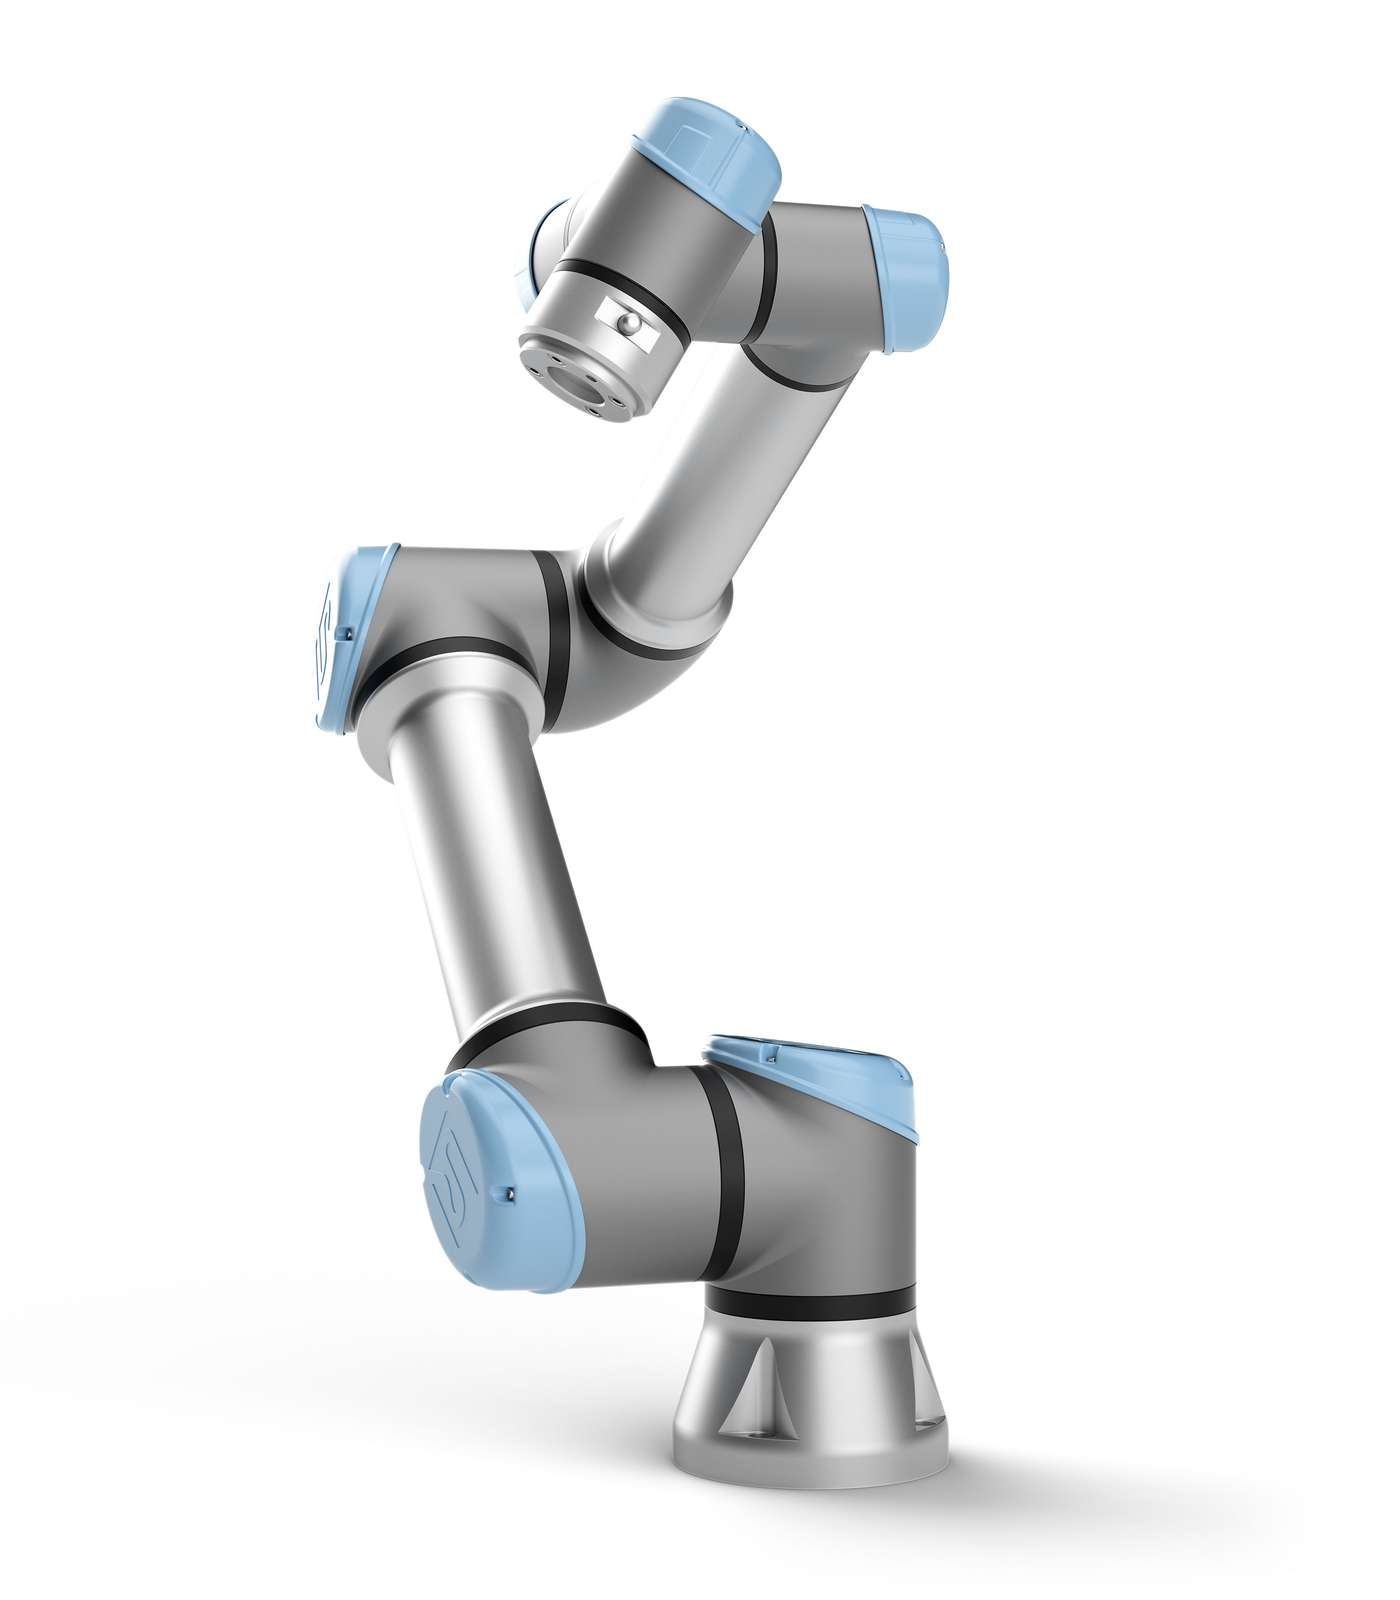
\includegraphics[width=0.4\linewidth]{figs/ur5.jpg}
    \caption{Universal Robots UR5 cobot - \cite{jugardUniversalRobots}} 
    \label{fig:ur5}
\end{figure} 

% \subsubsection{Distinguishing Cobots from Industrial Robots}

Cobots differentiate themselves from traditional industrial robots by prioritizing safety, ergonomics, and user accessibility. Unlike conventional robots that require extensive safety enclosures, cobots are equipped with advanced features such as force and torque sensors, vision systems, and anti-collision mechanisms. These capabilities enable them to operate safely in close proximity to humans without the need for restrictive barriers \cite{cobots-design}. The inherent design of cobots supports flexibility and ease of deployment, avoiding the high costs and complexity associated with retrofitting traditional robotic systems for similar functionality.

% \subsubsection{Economic and Practical Advantages of Cobots}

The adoption of cobots in industrial settings is driven by a combination of economic, operational, and health-related factors:
\begin{itemize}
    \item \textbf{Cost Efficiency:} Cobots can significantly reduce labor costs by performing repetitive tasks, thereby lowering direct unit production costs compared to traditional automation solutions \cite{cobot-2019collaborative}.
    \item \textbf{Enhanced Workplace Safety:} Their design minimizes occupational hazards, which leads to improved worker safety and health, addressing ergonomic challenges in manual labor.
    \item \textbf{Spatial Efficiency:} The compact and flexible nature of cobots allows them to be easily relocated and reconfigured within different production areas, optimizing factory space utilization \cite{cobots-implementation}.
\end{itemize}


These attributes are particularly beneficial in high-risk applications and industries that demand frequent changes in production layouts, such as electronics, automotive, and aerospace manufacturing.

When assessing the applicability of cobots versus traditional robots, several distinctions emerge. Cobots excel in tasks that require adaptability and human-like dexterity, such as assembly, placement, handling, and quality inspection. Their versatility and ease of integration make them suitable for low-volume, high-mix production environments, where agility is crucial. However, traditional robots retain an advantage in scenarios that demand high payload capacity, speed, and precision, particularly in heavy-duty manufacturing applications \footnote{\url{https://www.fanuc.eu/it/en/robots/robot-filter-page/m-2000-series}, acessed in 2024-09-22} \cite{robotics8040100}.


Despite their advantages, integrating cobots into existing workflows poses challenges. Issues such as interoperability with legacy systems, programming complexity for non-standard tasks, and optimizing cobot performance in dynamic environments require further research and development. Additionally, advancements in artificial intelligence and machine learning could unlock new capabilities for cobots, enabling them to autonomously adapt to changing tasks and work conditions, thereby extending their utility beyond predefined, structured environments.


\subsubsection{Future Trends in Human-Robot Collaboration}

According to the 2019 article \textit{Human–Robot Collaboration in Manufacturing Applications: A Review} \cite{robotics8040100}, future directions in 
\ac{HRC} are evolving due to advancements in cobot technologies, sensing methodologies, and algorithmic developments. The key trends identified include:

\begin{itemize}
    \item \textbf{Enhanced Scene Understanding:} Next-generation \ac{HRC} systems will prioritize deeper contextual awareness of the workspace and tasks at hand. This involves not only detecting the physical environment but also interpreting operator intentions, recognizing task progression, and continuously monitoring environmental dynamics. Such enhanced scene understanding will enable robots to anticipate human actions, predict potential safety risks, and adjust their behavior accordingly, thus fostering a higher level of operational safety and efficiency.

    \item \textbf{Advanced Sensing and Data Fusion:} To facilitate this enhanced scene understanding, advanced sensing methodologies and sophisticated data fusion techniques will be critical. By integrating multi-modal sensor data—such as visual, tactile, and auditory inputs—robots will be able to construct more comprehensive models of their surroundings and human collaborators. Real-time fusion of such data will allow systems to process information more effectively, ensuring safer interactions by preempting hazardous movements and improving overall system transparency. This, in turn, will enhance user trust and accelerate the adoption of HRC solutions across industries.

    \item \textbf{Integration of Learning Techniques:} 
    The incorporation of \ac{ML} and adaptive learning algorithms into \ac{HRC} systems represent a transformative leap forward. Techniques such as learning-by-demonstration, and \ac{RL} will enable robots to more accurately mimic human dexterity and decision-making processes, allowing them to learn from human input and adapt to non-repetitive, complex tasks. These adaptive systems will continuously improve based on interaction data, leading to more intuitive and efficient \ac{HRC} in dynamic industrial environments.

    \item \textbf{Improved Task Planning and Adaptive Learning:} Future \ac{HRC} systems will be distinguished by advanced task planning capabilities, driven by more sophisticated task modeling and real-time adaptation mechanisms. As robots become more capable of autonomously learning from both structured and unstructured environments, their ability to handle a wider array of tasks will expand, reducing human involvement in routine planning stages. The deployment of these capabilities in manufacturing and service sectors will enable robots to shift between tasks seamlessly, dynamically adjusting their behavior to respond to real-time changes in production or workflow.

    \item \textbf{User-Friendly Interfaces and Interaction Methods:} As the complexity of \ac{HRC} systems increases, the need for intuitive and accessible human-robot interfaces will become paramount. Developing user interfaces that enable seamless human control without requiring advanced technical expertise is a key area of research. Implementing \ac{AR} and \ac{VR} technologies is expected to play a pivotal role in this domain, offering operators immersive and intuitive control mechanisms. These interfaces will reduce cognitive load and enable operators to interact with robots more effectively, thus improving operational efficiency and overall system usability.
\end{itemize}


Historically, the focus has been on increasing the relevance of \ac{HRI} by addressing higher safety requirements and enabling 
robots to perform more complex tasks. Recently, the scope has expanded to include more sophisticated methods aimed at enhancing system performance, 
applying these methods across different application fields and tackling more intricate tasks. This expansion is driven by the emergence of new 
cobots, advancements in sensing technologies, matured algorithms, and accumulated experience in designing collaborative workcells \cite{robotics8040100}.



%%%%%%%%%%%%%% 16set 18h04 a parte abaixo, está ok ver so se é preciso adicionar mais alguma figura
\section{Digital Realities} 

\ac{DR's} encompass a spectrum of technologies that blend virtual elements with the real world to varying degrees. 
In 1994, Milgram and Kishino introduced the Reality-Virtuality Continuum, represented in figure \ref{f:real-virtual-continuum}, which outlines four key stages: Reality, \ac{AR}, \ac{AV}, and \ac{VR} \cite{milgram1994}.

\begin{figure}[h]
    \centering
    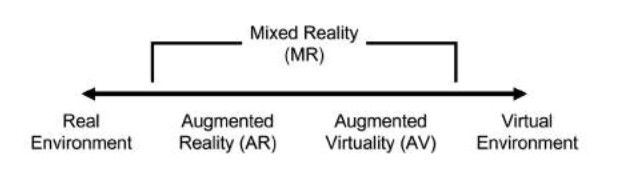
\includegraphics[width=0.6\linewidth]{figs/mixed-reality-continuum.jpg}
    \caption{Reality-Virtuality Continuum, from \cite{milgram1994}}
    \label{f:real-virtual-continuum}
\end{figure}

Reality corresponds to the perception of an unaltered physical environment.

\subsubsection{Augmented Reality (\ac{AR})}
    \ac{AR} enhances the user's perception of the real world by overlaying digital content such as 3D graphics, information, or media directly 
    onto their physical surroundings \cite{liu2022digitaltwin}. 
    This technology enables the virtual content to interact dynamically with the environment in real-time, with the ideal outcome being for users
    to perceive both virtual and real entities as inhabiting the same shared space, creating a unified and interactive experience \cite{Azuma1997}.
    \ac{AR} requires spatial registration to ensure that virtual additions are contextually and spatially aligned with the physical world.

    Typical \ac{AR} devices include \ac{AR}-\ac{HMDs}, tablets, \ac{HUDs}, projectors, \ac{VR} headsets with cameras (often referred to as pass-through or see-through VR) and 2D screen-based augmentation. Each device offers varying levels of environmental awareness, human interaction capabilities (such as hand tracking) and holographic projection features.


    A prime example of \ac{AR} is Pokémon GO, where virtual creatures known as Pokemons appear as if they exist within the real world, as shown in picture
    \ref{f:pokemon-go}, allowing users to interact with them through their mobile devices \cite{whatismixedreality}.

    \begin{figure}[h]
        \centering
        
\includegraphics[width=0.6\linewidth]{figs/mewtwo.jpg}
        \caption{Pokémon GO - an example of \ac{AR} application}
        \label{f:pokemon-go}
    \end{figure}


\subsubsection{Virtual Reality (\ac{VR})}
    
    \ac{VR} stage in the Reality-Virtuality Continuum represents a complete replacement of a user’s perception of the real world with a fully synthetic environment isolating them from the physical world \cite{milgram1994}.

    This immersion can also be achieved through \ac{HMDs} that consist on wearable devices that either project images directly into the user's eye or display them on a small screen positioned near the eye, such as the Oculus Quest 2.
    %  depicted in figure \ref{f:quest-2-vr}. 
    Some of these technologies are equiped with features like head tracking, enhancing the experience by allowing natural movements to influence the virtual environment.
    
    \ac{VR} typically allows for individual experiences and can transport users to remote or imaginary locations, offering a profound sense 
    of presence in a digitally constructed reality \cite{whatismixedreality, 8712803}.
    
    % \begin{figure}[h]
    %     \centering
    %     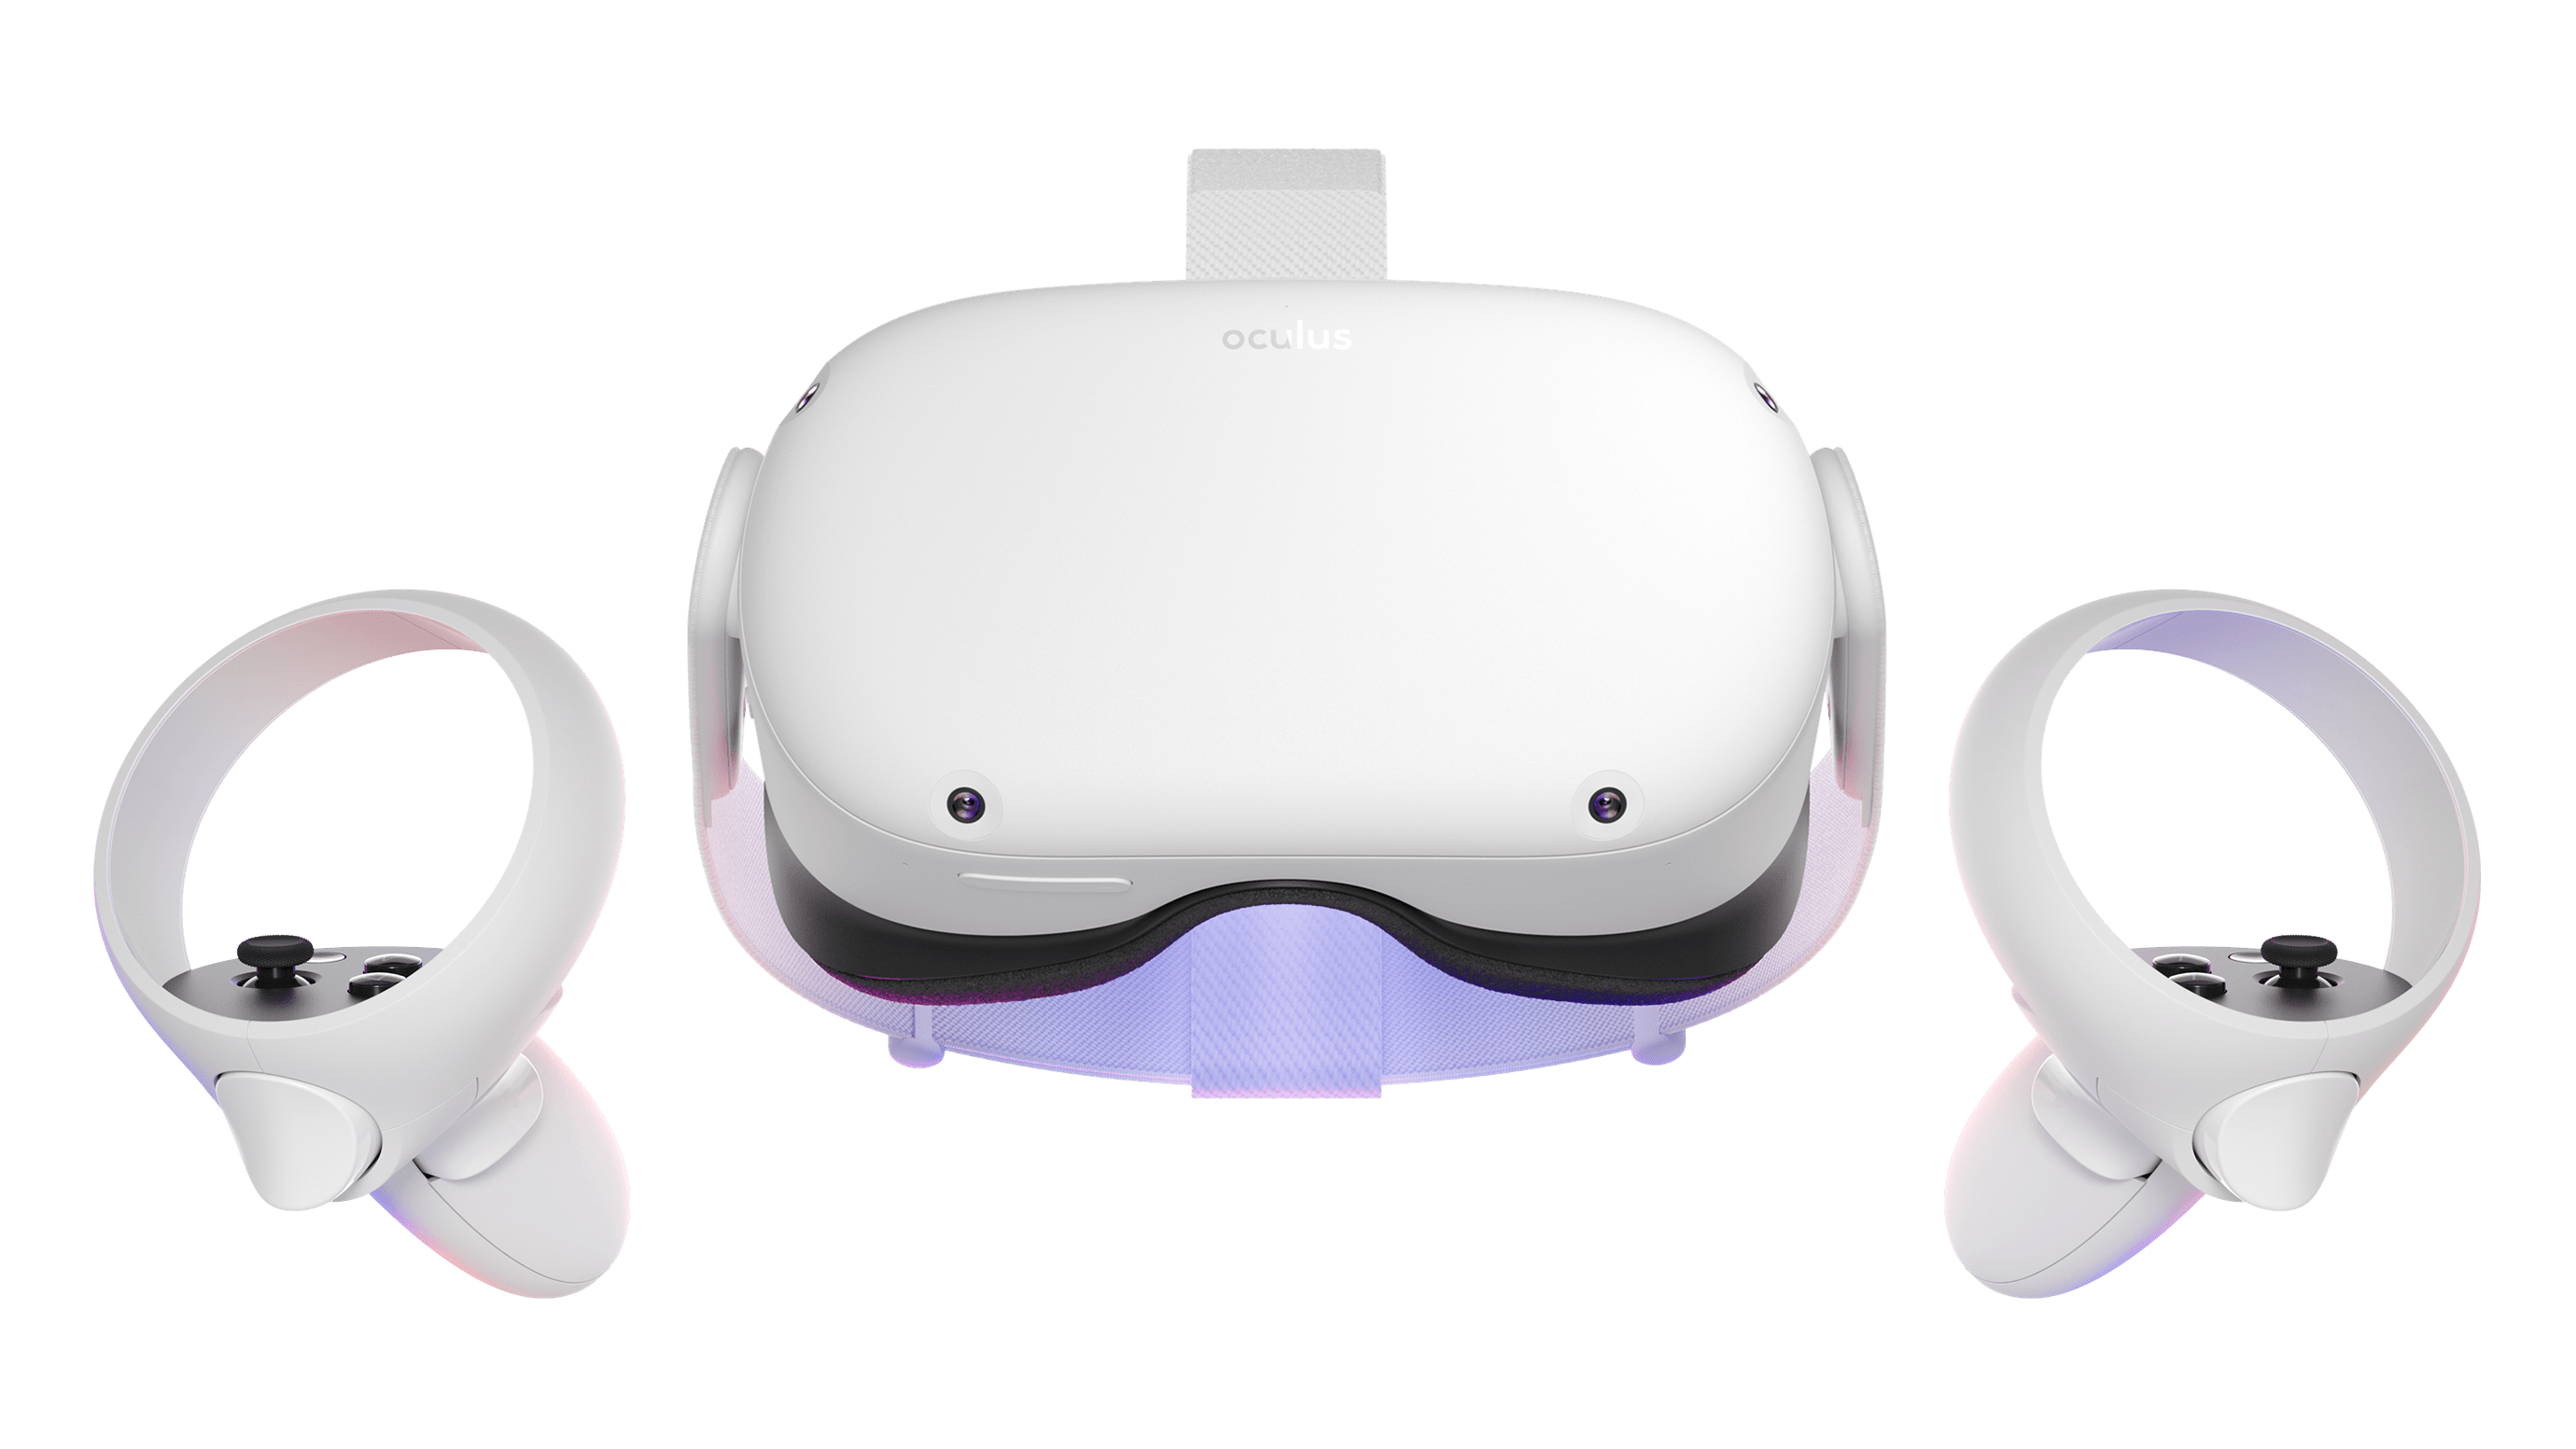
\includegraphics[width=0.6\linewidth]{figs/oculus-2-vr.png}
    %     \caption{Oculus Quest headset}
    %     \label{f:quest-2-vr}
    % \end{figure}

\subsubsection{Mixed Reality (\ac{MR})}

    Since \ac{MR} lacks a universally agreed-upon definition, various sources describe it in different ways. 
    According to Milgram and Kishino, \ac{MR} represents the merging of \ac{AR} and \ac{AV} technologies, creating environments where digital and physical elements interact fluidly \cite{milgram1994}. 
    In \cite{microsoft_mixed_reality}, \ac{MR} encompasses a spectrum, as depicted in the picture \ref{f:mixed-spectrum}, that includes everything
    from \ac{AR}, where the physical reality is dominant, to augmented virtuality, where virtual elements are more prominent, facilitating a seamless
    transition between real and virtual worlds.

    \begin{figure}[!htpb]
        \centering
        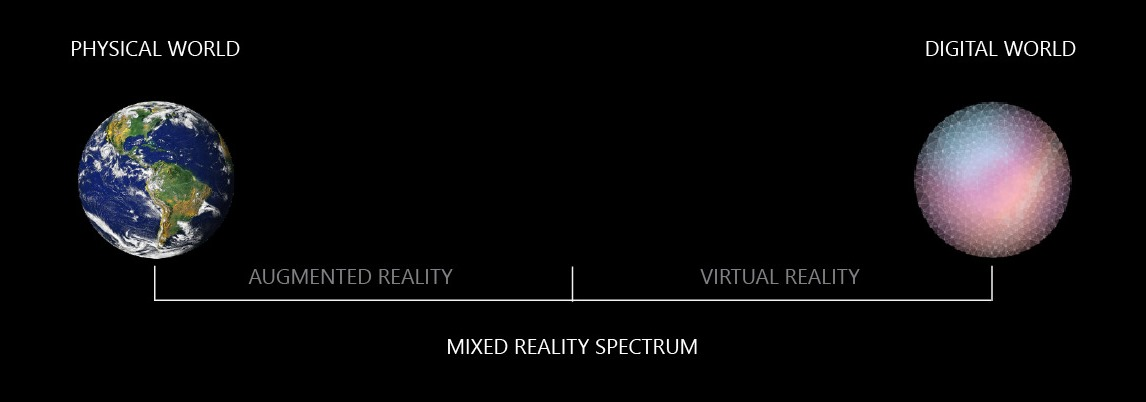
\includegraphics[width=0.8\linewidth]{figs/mixed-reality-spectrum.jpeg}
        \caption{The mixed reality spectrum, from \cite{microsoft_mixed_reality}}
        \label{f:mixed-spectrum}
    \end{figure}
    
   

    Speicher, Hall, and Nebeling (2019) argue that there is no universally agreed-upon definition of \ac{MR}, and instead, they identified six competing notions from both literature and expert interviews.
    Some define \ac{MR} as including collaboration between users in different realities, while some regard it as an advanced form of \ac{AR} where interactions with and within the environment are more complex. In some contexts, \ac{MR} is considered synonymous with \ac{AR}, while in others, it is seen as a distinct integration of both \ac{AR} and \ac{VR} technologies \cite{whatismixedreality}. 

    % Given that \ac{MR} is not a universally agreed concept, it can encompass a wide range of notions, including:
    % \begin{itemize}
    %     \item \textbf{\ac{MR} as a continuum}: Involving a range of experiences from \ac{AR} to augmented virtuality, depending on the degree of
    %     virtual content integrated into the real world.
    %     \item \textbf{\ac{MR} as Collaboration}: Describes the interactive processes between users in different realities, such as one in \ac{AR}
    %     and another in \ac{VR}, emphasizing the collaborative potential of \ac{MR} in shared or interconnected spaces.
    %     \item \textbf{\ac{MR} as Strong \ac{AR}}: Viewing \ac{MR} as an advanced form of \ac{AR} where interactions with and within the environment are 
    %     more complex and integrated.
    %     \item \textbf{\ac{MR} as a Synonym for \ac{AR}}: In this usage, the terms \ac{MR} and \ac{AR} are used interchangeably.
    %     This approach typically occurs when a system or experience aligns closely with \ac{AR}, and the definition of \ac{AR} is utilized to clarify what is 
    %     meant by \ac{MR}.
    %     \item \textbf{\ac{MR} as a Combination of \ac{AR} and \ac{VR}}: This definition describes \ac{MR} as an integration of both \ac{AR} and \ac{VR} technologies. 
    %     It refers to systems or applications that feature distinct \ac{AR} and \ac{VR} components, which may interact but are not necessarily seamlessly integrated.
    %     This can also apply to devices or apps capable of switching between \ac{AR} and \ac{VR} modes as needed.
    %     \item \textbf{\ac{MR} as an Alignment of Environments}: This concept of \ac{MR} involves the synchronization or alignment of virtual and physical 
    %     environments. It describes systems where the virtual and real components are distinct yet aligned, similar to how collaboration setups 
    %     work but without requiring actual collaborative interactions or physically separate environments.
    % \end{itemize}

\subsubsection{Extended Reality (\ac{XR})}
    The term \ac{XR} serves as an umbrella concept that includes \ac{AR}, \ac{MR}, and \ac{VR} as distinct but related technologies. It encompasses technologies designed to enhance sensory experiences by blending the physical and digital worlds \cite{pesca2021augmented}. These technologies allow users to engage with virtual and augmented elements in varying degrees, depending on the specific application or device in use.


% use this? - 17 set 00h18
% Therefore, it holds great promise for enhancing collaborative efforts, particularly in remote interactions, where \ac{AR} is utilized by for 
% on-site members, overlaying digital information onto the physical environment, and \ac{VR} is employed for remote members, immersing them in 
% a simulated virtual environment. This integration of both digital realities allow participants from different locales to share a common virtual 
% space for interaction.

%%%%%%%%%%%%%%    % 16 set 18h04  a parte acima esta ok, ver so se é preciso adicionar mais alguma figura

%%%%%%%%%%%%%% é preciso entrar em mais detalhe sobre o que é MR e como se enquadra no contexto de HRC????? faz sentido? - do artigo de mixed realities
%%%%%%%%%%%%%% capitulo 8 - a conceptual framework for mixed reality . 16 set 18h04
    % \subsection*{Summary of Mixed Reality Concepts}

    % The landscape of \ac{MR} is notably fragmented, influenced by diverse expert opinions and various scholarly sources. 
    % Despite these differences, there is a consensus on the utility of a unified definition for clarity, particularly within Human-Computer Interaction 
    % research. However, the approach adopted does not seek to establish a singular definition but rather to accommodate the variety of existing perspectives.
    
    % \subsection*{Conceptual Dimensions of MR}

    % Several dimensions have been identified to classify \ac{MR} experiences more clearly:

    % \begin{itemize}
    %     \item \textbf{Number of Environments:} This dimension addresses the count of physical and virtual environments involved in \ac{MR} experiences. 
    %     For instance, a \ac{VR} experience might be considered a separate environment even when occurring in the same physical space as an \ac{AR} setup.
    %     \item \textbf{Number of Users:} Reflects the user involvement needed for different types of \ac{MR}. While the collaboration type of \ac{MR} 
    %     typically involves multiple users, other forms might not.
    %     \item \textbf{Level of Immersion:} Describes the depth of immersion, which varies independently from the level of virtuality. This is crucial 
    %     for understanding user engagement in \ac{MR} environments.
    %     \item \textbf{Level of Virtuality:} Indicates the extent of virtual content integrated into the user's perception. It parallels the 
    %     Reality-Virtuality Continuum and varies from non-existent to fully virtual.
    %     \item \textbf{Degree of Interaction:} Categorized into implicit and explicit interactions, this dimension focuses on how users interact 
    %     with the \ac{MR} system—ranging from passive engagement to active manipulation of the \ac{MR} scene.
    % \end{itemize}

    % \subsection*{Additional Dimensions}

    % \begin{itemize}
    %     \item \textbf{Input:} Encompasses non-interactive inputs like motion tracking, geolocation, and sensor data, which inform the \ac{MR} environment.
    %     \item \textbf{Output:} Involves the types of sensory feedback provided to the user, potentially including visual, auditory, haptic, and other sensory outputs.
    % \end{itemize}

    % These dimensions form a framework that allows for a structured classification and discussion of \ac{MR} experiences, accommodating the range of definitions and applications highlighted by industry and academic experts.

% \subsection{Extended Reality}  -------------- perguntar ao eurico e bernardo se é preciso falar disto ou fica apenas pela mixed reality?
% % - importante para a industria 4.0
% % mencionar áreas de aplicacao onde ja existe.
% % dar + enfase aos trabalho alinhados com HRC e HRI
% \ac{XR} is a recent comprehensive term that encapsulates all immersive technologies, including \ac{VR}, \ac{AR}, and \ac{MR}. 
% These technologies extend the spectrum of human experience by merging the digital and physical realms in various degrees and forms. 

% \ac{XR} technologies are pivotal in:
% \begin{itemize}
%     \item creating a continuum of immersive experiences, ranging from fully virtual environments to the enhancement of the physical world with 
%     digital overlays \cite{Morimoto2022}.
%     \item transforming the manufacturing industry by enhancing visualization, training, and operational efficiency.
% \end{itemize} 

% \subsection{Limitations of XR}

% While \ac{XR} holds great promise for revolutionizing remote interactions, it also has challenges, especially in distant settings.

% It begins with the limitation in perspective and environmental context. The view available to remote participants is restricted to what their on-site 
% counterparts can share, which may limit a full understanding of the environment. This constraint can lead to less effective guidance and decision-making 
% from afar. 

% Moreover, \ac{XR} technologies often emphasize sharing visual and audio data, neglecting the collection of multisensory information. 
% This lack of comprehensive data collection prevents remote participants from fully grasping the nuances of the physical location, missing out 
% on critical contextual cues necessary for a deep understanding of on-site conditions.

% Additionally, the interaction with physical objects through \ac{XR} can be superficial, lacking the depth needed for intricate explanations or 
% precise gestures, especially in complex or dynamic situations. This limitation can make it challenging to perform tasks that require detailed 
% manipulation.

% Furthermore, navigation poses another challenge for on-site users, particularly in environments that are complex or fraught with hazards. 
% The difficulty in moving safely and efficiently through such spaces can compromise the sharing of contextual information and hinder the overall 
% effectiveness and efficiency of the tasks being done.

% These limitations underscore the need for ongoing advancements in \ac{XR} technology to address these gaps and fully leverage its potential in 
% remote collaboration \cite{Lambrecht2021,Suzuki2022}.



%%%%%%%%%%%%%%%%%%%%%%%%%%% abaixo - verificar se alguma informacao daqui pode ser util para os DT - 19 set 16h11 %%%%%%%%%%%%%%%%%%%%%%%%%%% 

% 19 set 00h14 - parte dos dt parece estar ok (falta adicionar figuras e tabelas) - ordenar melhor ( ver o que o chat deu)
% - a seguir falar das solucoes industriais - ar e dt para remote collaboration
% introduzir human robot collaboration antes? 
% \section{Digital Twins}
% cite from article - "state of art survey digital twin implementations" 

% \ac{DT} are virtual replicas of physical entities, enabling the simulation, analysis, and control of systems in a digital realm. 
% Their importance in enhancing \ac{HRC} lies in their ability to provide a real-time, interactive environment that mirrors the 
% physical world, allowing for improved decision-making, efficiency, and flexibility in industrial applications.

% By transforming smart manufacturing, \ac{DT} enable comprehensive examination and prediction of physical systems' behaviors, 
% optimizing operations and minimizing downtime. In \ac{HRC}, \ac{DT} significantly boost ergonomic interactions, adapting robotic movements to meet 
% human needs and constraints, thereby ensuring a safer and more productive workplace \cite{Tao2019}.

% The integration of \ac{DT} in various fields is supported by advancements in big data and \ac{IoT}, providing the necessary infrastructure for its 
% implementation. As a cutting-edge technology, \ac{DT} leverages modern data surges to assist engineers, managers, healthcare professionals, and 
% policymakers in managing complex systems such as production lines, healthcare, and smart cities (citar 4-8 confirmar quais os casos aplicaveis aqui).
% These systems offer high fidelity monitoring, diagnostics, and prognostics tools, enhancing operational oversight and decision-making processes.

% Moreover, \ac{DT} are instrumental in the proactive management of \ac{HRC}, fostering mutual-cognitive, predictable, and self-organizing functionalities that 
% enhance the efficiency and safety of \ac{HRI} \cite{Li2023}.

% Originally conceptualized by NASA in the 1980s, the idea of \ac{DT} was intended to monitor spacecrafts from Earth. This concept has evolved significantly 
% with the advancements in computational and \ac{IoT} technologies. Modern \ac{DT} systems utilize real-time data from sensors to accurately reflect the 
% state of the physical twin, enhancing the fidelity and applicability of simulations (cite 10).

% Nowadays, a notable implementation of \ac{DT} technology is observed in Singapore's Smart Nation Initiative, where the Land Transport Authority is developing a 
% \ac{DT} of the country to inform policy decisions by testing potential policies virtually before they are enacted. This application not only demonstrates
% the immense potential of \ac{DT} for contemporary and future technologies but also underscores the ongoing commitment to advancing this concept (cite 6).

% However, the concept of \ac{DT} lacks a standardized definition, leading to a variability in the scope and execution of \ac{DT} implementations. 
% The dual nature of cyber and physical components in \ac{DT} makes \ac{AR} a suitable companion for visualizing and interacting with these complex 
% systems (cite the article itself).

% As \ac{DT} technology continues to attract interest, the necessity for intuitive data visualization methods becomes apparent. Non-expert users must 
% be able to understand and interact with the complex data provided by \ac{DT} systems effectively. \ac{AR} offers a promising solution by overlaying 
% virtual data directly onto physical objects, providing a more natural and intuitive user interface for interacting with digital 
% information cite(12).
% \ac{AR} expands the traditional interaction from 2D screens to 3D real-world applications, making it an ideal tool for enhancing user interaction 
% with digital twins. By enabling users to view and interact with maintenance instructions projected directly onto equipment, \ac{AR} facilitates more 
% efficient and effective operation and maintenance processes (cite 13).



% \subsection*{Digital Twins in Academia and Industry}
% The term \ac{DT} is widely recognized in both academic and industrial circles as a \ac{CPS} that typically consists of three main components: 
% \begin{itemize}
%     \item A physical system.
%     \item A virtual model.
%     \item The connections between them (cite 1,2,3 from the dt article).
% \end{itemize}

% Research applications of \ac{DT} span across 
% various fields, offering solutions for lifecycle management, \ac{PHM}, and urban planning, to name a few (cite 4-8).

% Critically, the industry's adoption of \ac{DT}, led by companies like Siemens, often focuses on creating digital shadows rather than true \ac{DT}, 
% characterized by a lack of bidirectional communication. True \ac{DT} systems are distinguished by their ability to not only update the virtual model 
% based on changes in the physical system but also to allow alterations in the virtual model to affect the physical entity (cite 9- add table 5).

%%%%%%%%%%%%%%%%%%%%%%%%%%% acima - verificar se alguma informacao daqui pode ser util para os DT - 19 set 16h11 %%%%%%%%%%%%%%%%%%%%%%%%%%% 

%%%%%%%%%%%%%%%%%%%%%%%%%%% abaixo - parte a usar para DT - 19 set 16h11 %%%%%%%%%%%%%%%%%%%%%%%%%%%%%%%%%%%%%%%%%%%%%%%%%%%%%%  

\section{Digital Twins}

% \subsubsection{Introduction to Digital Twins}
Digital Twins (\ac{DTs}) are sophisticated virtual replicas of physical entities that enable simulation, analysis, and control of systems within a digital framework. 
These digital counterparts are pivotal in enhancing \ac{HRC}, as they provide real-time, interactive environments that mirror the physical world. 
This mirroring capability facilitates improved decision-making, efficiency, and flexibility across various industrial applications.

% \subsubsection{Historical Origins of Digital Twins}
The concept of \ac{DT} was originally formulated by NASA in the 1980s for monitoring spacecrafts from Earth. With advancements in \ac{IOT} and 
computational technologies, modern \ac{DT} systems now utilize real-time sensor data to enhance the accuracy and reliability of simulations, 
significantly evolving from their initial conception \cite{liu2022digitaltwin}.

% \subsubsection{Characteristics and Applications of Digital Twins}
\ac{DT} transform smart manufacturing by enabling detailed examination and prediction of the behavior of physical systems, thereby optimizing operations 
and minimizing downtime. In the realm of \ac{HRC}, \ac{DT} significantly enhance ergonomic interactions by adapting robotic movements to meet human needs,
thus ensuring safer and more productive workplace conditions \cite{8477101}.

A notable implementation of \ac{DT} technology can be observed in Singapore's Smart Nation Initiative, where the Land Transport Authority 
utilizes a \ac{DT} to simulate and evaluate potential policies before implementation, showcasing the vast potential of \ac{DT} for modern and 
future technologies \cite{isprs-archives-XLII-4-W7-37-2017}.

\subsubsection{Digital Twins in Academia and Industry}

Digital Twins (DT) have gained significant traction in both academic research and industrial applications in recent years. Despite their growing prominence,
there is no universally accepted formal definition of a DT. 

Nevertheless, the majority of reputable researchers concur that a DT is a \ac{CPS} comprising at
least three essential components: 
\begin{itemize}
    \item A physical system,
    \item A virtual model,
    \item Connections facilitating bidirectional communication between the physical and virtual models \cite{TaoFei, 8477101, ROSEN2015567}.
    % confirm these citations above
\end{itemize}

In academic settings, DTs have been explored across a wide array of applications, including machine tool life management, product health management,
smart cities, and patient health monitoring, among others \cite{8361285, TAO2018169, isprs-archives-XLII-4-W7-37-2017, 10.1007/978-3-030-23162-0_19, 6296978}. These applications demonstrate the versatility and potential of DTs in enhancing efficiency, predictive maintenance, and system optimization. 
% confirm these citations above

In the industrial sector, numerous companies, such as Siemens, offer software and platform solutions aimed at creating DTs for their industrial partners. 
However, some critics argue that these solutions represent digital shadows rather than true DTs. 

The primary contention is the lack of bidirectional communication capabilities, specifically, while changes in the physical system can influence the virtual model, the reverse—where modifications in the virtual model impact the physical system—is often absent \cite{CIMINO2019103130}. 

Figure \ref{f:dt-structure}, \cite{dt_model} outlines the \ac{DT} reference model, illustrating the bidirectional communication between the physical 
and digital entities. This configuration underscores the distinction between true DTs and digital shadows, the latter often criticized for lacking 
interactive communication capabilities \cite{CIMINO2019103130}.

\begin{figure}[!htpb]
    \centering
    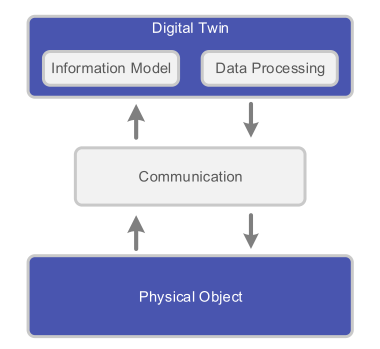
\includegraphics[width=0.4\linewidth]{figs/dt_reference_model.png}
    \caption{A Digital Twin reference model \cite{dt_model}}
    \label{f:dt-structure}
\end{figure}

% However, the concept of \ac{DT} lacks a standardized definition, leading to a variability in the scope and execution of \ac{DT} implementations. 
% The dual nature of cyber and physical components in \ac{DT} makes \ac{AR} a suitable companion for visualizing and interacting with these complex 
% systems (cite the article itself).

As emphasized by Liu et al.~, "A true DT must include bidirectional communication instead of having a virtual model that updates
according to a physical system." 
Given that the concept of \ac{DT} lacks a standardized definition, leading to a variability in the scope and execution of \ac{DT} implementations and
defining a misconception, the critical distinction between three types of interaction is further ilustrated in Table ~\ref{tab:levels_of_control}, ~\cite{liu2022state}.
% This critical distinction is further illustrated in Table~\ref{tab:levels_of_control}.

\begin{table}[!htpb]
    \centering
    \caption{Levels of Control, adapted from \cite{liu2022state}}
    \label{tab:levels_of_control}
    \begin{tabular}{@{}l>{\raggedright\arraybackslash}p{10cm}@{}}
    \toprule
    Level of Interaction & Description \\ 
    \midrule
    No interaction & Virtual model and physical system are not connected through a network. The virtual model only simulates and models a physical 
    system without any real-time updates. \\ \hline
    Unidirectional & The physical system feeds sensor data to the virtual model through a network. The virtual model utilizes data to update the 
    current state and predict future states. \\ \hline
    Bidirectional & Both the physical system and the virtual model can send data to each other. The virtual model updates using physical data while 
    the physical system can be controlled through data sent by the virtual model. \\ 
    \bottomrule
    \end{tabular}
\end{table}



\subsubsection{Integration of Augmented Reality with Digital Twins} % verify this section references - if it matches what it said - 23 set 19h56
The integration of \ac{AR} with \ac{DT} represents a significant advancement in enhancing user interactions with complex systems. 
\ac{AR} overlays virtual data directly onto physical objects, thereby providing a more intuitive and engaging interface for users. 
This capability is particularly beneficial in industrial settings where \ac{AR} can facilitate more efficient and effective operation and 
maintenance processes \cite{article12, peddie2017augmented}.

Despite the numerous advantages of \ac{DT}s, a significant challenge lies in the effective visualization of the complex data they generate. 
As interest in \ac{DT}s grows, it becomes increasingly important to provide users with intuitive and accessible methods to interpret and interact 
with this data. According to \cite{article12}, the benefits of real-time data and information provided by \ac{DT}s cannot be fully realized without 
proper visualization techniques that present complex information in a clear and uncluttered manner, especially for users with limited technical expertise.

\ac{AR} offers a promising solution to this challenge by enhancing data visualization and user interaction. Traditionally, users interact with digital 
information through 2D interfaces such as screens and monitors. However, \ac{AR} expands this interaction into the real world by overlaying virtual 
data onto physical objects, creating immersive 3D experiences that align with users' familiar environments \cite{peddie2017augmented}. This 3D visualization enables
users to better understand and absorb information through visual cues, which are often more effective than textual or auditory information \cite{article-teaching}.
For instance, projecting maintenance instructions directly onto a machine allows users to perform maintenance tasks more efficiently compared to 
consulting physical manuals \cite{inproceedings}. Moreover, \ac{AR} has been successfully utilized in various manufacturing processes to provide guidance 
for maintenance procedures and to train novice workers, demonstrating its versatility and effectiveness in industrial settings \cite{ong2004virtual}.

By integrating \ac{DT} with \ac{AR}, it is possible to monitor the state of a system in real-time while simultaneously displaying relevant
data and information through \ac{AR} interfaces. This integration not only enhances the user experience but also improves operational efficiency and 
safety by providing actionable insights in an intuitive and accessible manner.

\section{Human-Robot Collaboration in Industrial Applications}
Following the detailed exploration of \ac{DT} and \ac{AR}, this section discusses how these technologies integrate into \ac{HRC}, demonstrating significant improvements in interaction, safety and efficacy in practical examples from industry solutions with specific emphasis on remote collaboration.

\subsubsection{Enhancing Human-Robot Collaboration (\ac{HRC}) through Augmented Reality (\ac{AR}) and Digital Twin (\ac{DT}) Implementation}

\begin{enumerate}
    \item \textbf{Augmented Reality for Enhanced Interaction and Safety}
    % Augmented reality user interface design and experimental evaluation for human-robot collaborative assembly - reference : CHU2023313
    % Leveraging \ac{AR} can significantly improve the interaction between humans and robots by providing intuitive visualizations and reducing the need 
    % for continuous visual contact. As demonstrated by Chu et al. \cite{CHU2023313}, effectively conveying robot intentions through \ac{AR} visuals enhances 
    % worker awareness of their surroundings, thereby improving safety and efficiency in collaborative tasks. 
    
    % After analysing previous related work and implemented methodologies, 

    % The \ac{AR} interfaces clearly visualize the 
    % robot's work envelope, as depicted in Figure~\ref{fig:ar-envelope}, enabling human operators to navigate shared workspaces safely and efficiently.
    
    % \begin{figure}[htp]
    %     \centering
    %     \begin{subfigure}{.5\textwidth}
    %         \centering
    %         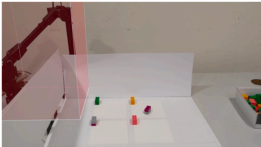
\includegraphics[width=0.9\linewidth]{figs/a-work-env.png}
    %         \caption{}
    %         \label{fig:sfig1}
    %     \end{subfigure}%
    %     \begin{subfigure}{.5\textwidth}
    %         \centering
    %         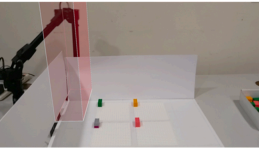
\includegraphics[width=0.9\linewidth]{figs/b-work-env.png}
    %         \caption{}
    %         \label{fig:sfig2}
    %     \end{subfigure}
    %     \begin{subfigure}{.5\textwidth}
    %         \centering
    %         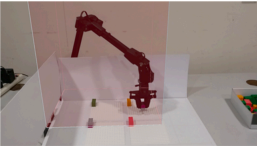
\includegraphics[width=0.9\linewidth]{figs/c-work-env.png}
    %         \caption{}
    %         \label{fig:sfig3}
    %     \end{subfigure}%
    %     \begin{subfigure}{.5\textwidth}
    %         \centering
    %         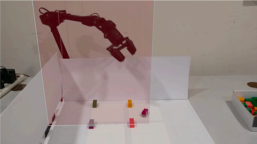
\includegraphics[width=0.9\linewidth]{figs/d-work-env.png}
    %         \caption{}
    %         \label{fig:sfig4}
    %     \end{subfigure}
    %     \caption{AR displayed work envelope of robotic arm \cite{CHU2023313}}
    %     \label{fig:ar-envelope}
    % \end{figure}
    

%     %notas para adicionar sobre o artigo - acima - 
%     The experiment aims to verify and
%     cross-compare the effectiveness of visual and haptic cues in various forms that convey the robot intent to human.
%     Analysis of the work performance and gazing behavior of participants shows that both cues can reduce their
%     visual attention on the moving robot during the collaboration. 
%     [10] emphasized the importance of human information
%     communication on assuring safety in HRC. They considered AR as an
%     ideal interface that enables the human and robot to ground their
%     communication and intentions by sharing an ego-centric view. AR also
%     allows for an exocentric view of the collaborative workspace that provides spatial awareness. This study suggested that a human-robot
%     collaborative system based on multimodal interactions would be more
%     effective and natural than unimodal.
%     Since  AR headsets still have a very limited field of view compared to the human vision. Visual guidance for localizing out-of-view objects in the limited display space often causes visual conflicts such as cluttering or occlusion of information [11]
%     Other works [12] proposed a visualization interface in AR HMD that superimposed the intended robot motion onto the user’s
%     view of real environment verifying that  the user determined where the robot was going to move using the interface more
%     quickly and accurately than 2D display or no assisted visualization.

%     the article itself outlines that providing AR user interfaces with either visual, haptic or multi-modal cues for HRC are benefitial.
%         Visual-based AR (cues) help overcome limitations arising from complex environments by superimposing visuals in an HMD without compromising robot mobility. this system also revealed to reduce the idle robot time as well as the task completion time when compared to the baseline without the user interface or the space sharing. However, user experience assessment showed that the HoloLens setup was not yet technically mature on the shop floor, particularly the limited field of view.
%         Visual feedback on a screen displayed the swept volume generated by the planned robot trajectory. Experimental data indicated that the human
%         workers felt more comfortable and had a better understanding of the robot motion and goals using multi-modal feedback. 
%         Haptic cues - It is sometimes advantageous in industrial environments over visual and auditory modalities, which could be overloaded or blocked on site. Vibrotactile devices have been applied to control industrial robot and to inform users of approaching singularities and joint limits in a factory [22]
%         Visual and acustic - aimed to reduce human's anxiety related to the unpredictability of the robot motion in a shared workspace. Acoustic feedback was used to alert the human when the robot had detected a possible collision and changed the planned motion.

%         % ROS was useful, said by this article, this reinforces that the model i developed goes in line to what the literature supports
%         Implementing the system using the Robot Operating System also allowed modularity and extendibility for such a multi-device and multi-user approach.

%         % see conclusion - were the visual and haptic cues that communicated the robot motion useful in a collaborative assembly for the user?

%         % experiment:
%         During the assembly, a human operator picks, fetches, and stacks LEGO blocks onto specific work areas determined by the block color, while a desktop robot transports extra blocks to the areas over a wall.

%         In addition, both visual and tactile cues are presented in two forms that convey the robot motion with different degrees of information in AR.

%         % display 
%         As shown in figure \ref{f:area-1}, the operator was collaborating with a robot arm in a 25 cm × 25 cm work space in the middle of the table. The space was divided into four areas and each held LOGO blocks of a different color (see Fig. 2). The robot arm was mounted outside of the work space separated by a wall.

%         \begin{figure}[!htpb]
%             \centering
%             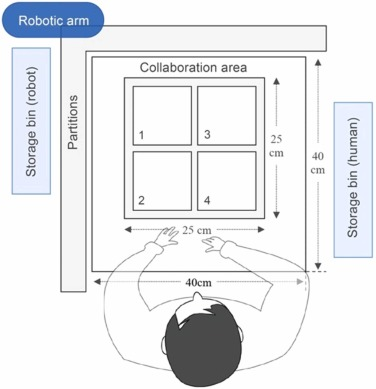
\includegraphics[width=0.4\linewidth]{figs/area-1.jpg}
%             \caption{Collaborative work space in the experiment, \cite{CHU2023313}}
%             \label{f:area-1}
%         \end{figure}

%         The space was divided into four areas and each held LOGO blocks of a different color (see figure \ref{f:robot-area-1}). The robot arm was mounted outside of the work space separated by a wall.

%         \begin{figure}[!htpb]
%             \centering
%             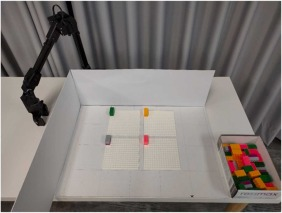
\includegraphics[width=0.4\linewidth]{figs/robot-area-1.jpg}
%             \caption{Actual work environment in the experiment, \cite{CHU2023313}}
%             \label{f:robot-area-1}
%         \end{figure}

%         The human and the robot independently performed individual tasks without a physical contact during the experiment. The operator picked up a block randomly from a storage bin on the right; then assembled the block into the area corresponding to its color. The storage bin contained 12 blocks of each different color. In contrast, the robot picked up a block at random times from the storage area on the left, which contained 4 blocks of each color. It then delivered the block to one of the four areas, also at random. The manual assembly of LEGO blocks must comply with the
%         following instructions. First, only one block was assembled at one time.
%         The operator could finish the assembly by using one or both hands.
%         Second, a block must be assembled to the area matching its color. The
%         block assembly started from the upper left of each area; then sequentially progressed from left to right and from up to bottom. Next, a block
%         could not be placed on top of existing blocks. The operator was asked to
%         complete the tasks as efficient as possible, while avoiding any collision
%         or physical contact with the robot.

% % visual and haptic user implemented interfaces
%         The visual interface was implemented in the HoloLens 2, which displayed the robot’s planned motion and the swept volume generated by the robot trajectory. The visual interface was designed to provide the operator with a clear understanding of the robot’s intended motion and goals. The haptic interface was implemented using the SenseGlove Nova™, which provided force feedback to the operator’s hand. The haptic interface was designed to alert the operator of the robot’s planned motion and to guide the operator’s hand to the correct assembly location. they can be seen in the figure \ref{fig:haptic-visual-cues}.

%         \begin{figure}[htp]
%             \centering
%             \begin{subfigure}{.5\textwidth}
%                 \centering
%                 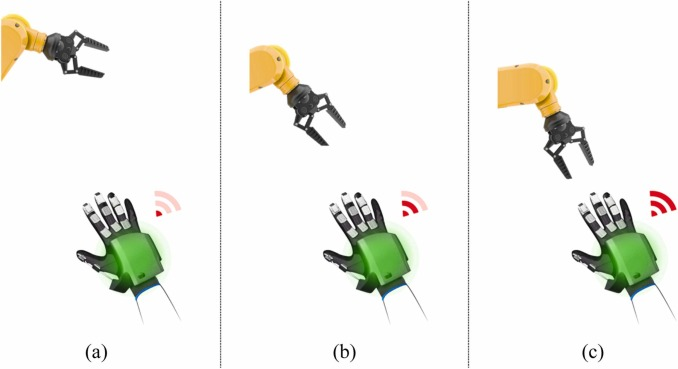
\includegraphics[width=0.9\linewidth]{figs/haptic-cues.jpg}
%                 \caption{Indicating the gripper’s destination using vibration on different human fingers.}
%                 \label{fig:sfig1}
%             \end{subfigure}%
%             \begin{subfigure}{.5\textwidth}
%                 \centering
%                 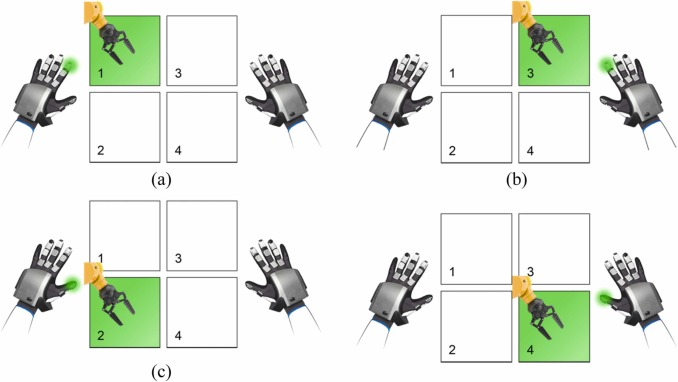
\includegraphics[width=0.9\linewidth]{figs/visual-cues.jpg}
%                 \caption{Indicating the proximity of gripper via change of vibration frequency.}
%                 \label{fig:sfig2}
%             \end{subfigure}
%             \label{fig:haptic-visual-cues}
%         \end{figure}
        

%         % AR interfaces - integration:
%         A WidowX 250 Robot Arm developed by Trossen Robotics was used
% in the experiment. This device is a 5-DOF desktop robotic arm with a
% 650-mm work range centered at the base. The robot
% control is realized by a computer through the Robot Operating System
% (ROS) [42]. ROS supports the motion planning framework MoveIt [43],
% which provides fundamental open-source functions for robot motion
% planning and manipulation. (this part is similar to the one of the project i am working with- robot with ROS and also Moveit integrated - useful to mention)
% the manual tasks were performed while wearing a Microsoft HoloLens 2: The two visual interfaces were mainly implemented in HoloLens 2.
% We adopted SenseGlove Nova™, shown in figure \ref{f:HTC-gloves} to produce force feedback required
% by the haptic user interfaces. It is a programmable device commonly
% used in \ac{VR} applications to simulate tactile perception for
% high interactivity. To integrate the device with AR applications involves
% recognition of the user’s hand gesture and position in real environment.
% For this purpose, a HTC VIVE tracker was attached on each glove.

% \begin{figure}[!htpb]
%     \centering
%     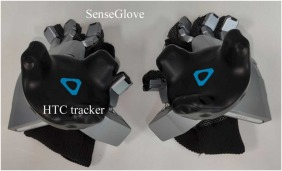
\includegraphics[width=0.6\linewidth]{figs/gloves.jpg}
%     \caption{Attaching HTC trackers on SenseGlove, \cite{CHU2023313}}
%     \label{f:HTC-gloves}
% \end{figure}

% Figure \ref{f:system-framework} shows the system framework proposed to integrate hardware
% devices with the UNITY engine residing on a desktop computer as an
% application server. The computer connected with the robot arm using a
% USB cable via Ubuntu v20.4 and executed motion control in ROS. It
% communicated with the HoloLens 2 and SenseGlove using WiFi and
% Bluetooth, respectively.

% \begin{figure}[!htpb]
%     \centering
%     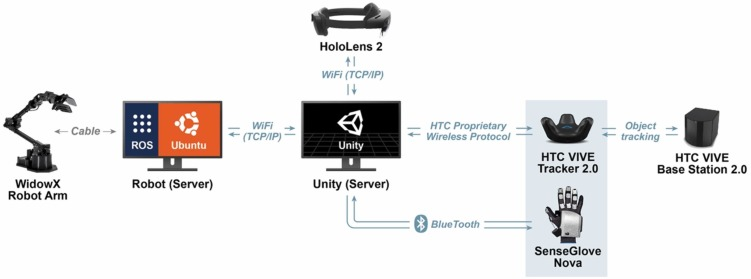
\includegraphics[width=0.6\linewidth]{figs/system-framework.jpg}
%     \caption{The system framework for integration of hardware devices in the experiment, \cite{CHU2023313}}
%     \label{f:system-framework}
% \end{figure}

% Section: Implementing AR and Digital Twins in Human-Robot Collaboration (HRC)


    The work reviewed several previous studies that gathered and exposed information on implementing \ac{AR} with \ac{DT}. Specifically, it integrates a real robot with visual and haptic \ac{AR} interfaces and explains their development. This section provides an overview of the implementation techniques, advantages, and experiment performed using these technologies in a collaborative LEGO assembly task.

    \paragraph{\textbf{\ac{AR} and \ac{HRC} Integration}}
    The article outlines that \ac{AR} interfaces with visual, haptic, acoustic, or multi-modal cues are beneficial for \ac{HRC}. \ac{AR} is considered an ideal interface to enhance human-robot communication by providing both ego-centric (ability to share remote views) and exocentric (ability to visualize the robot relative to the task space) views of the collaborative workspace, improving spatial awareness and interaction \cite{doi:10.5772/5664}. 
    
    It has been demonstrated that multimodal interactions, such as audio-tactile feedback, can significantly enhance the \ac{HRC} experience by making it more intuitive and effective. These multimodal approaches provide valuable insights that would otherwise be limited, such as overcoming the restricted \ac{FOV} in \ac{HMDs}.
    For instance, research has shown that while audio-tactile guidance might be slower compared to visual methods like EyeSee360, it offers a similar or even slightly better accuracy rate. Moreover, it can be especially beneficial for users with visual impairments, as the same information is conveyed through another sensory channel without degrading performance.

    Visual \ac{AR} cues, implemented via \ac{HMDs}, allow users to navigate complex environments by overlaying visual information without hindering the robot’s movement. However, challenges like the limited \ac{FOV} of devices like the HoloLens present obstacles in industrial settings.
    In scenarios where visual and auditory modalities are overwhelmed, haptic feedback provides a viable alternative. Vibrotactile devices, for instance, have been successfully used to alert operators about robot motion, approaching singularities, and joint limits in factory environments. Acoustic feedback also helps reduce human anxiety in shared workspaces by warning users of potential collisions or sudden changes in the robot’s trajectory \cite{9199570}.

    In a human-robot collaboration scenario, such as the one used in \cite{doi:10.1177/0018720814565188}, where two distinct modes for robot operation were implemented, standar and human-aware, users reported feeling safer when the mode was able to differentiate between user actions and the surrounding environment. 

    \paragraph{\textbf{Implementation Techniques}}
    The system was developed using the \ac{ROS} to control a WidowX 250 Robot Arm, which provided the flexibility and modularity required for a multi-device and multi-user setup. MoveIt framework  was used for robot motion planning and manipulation, aligning with the technical model proposed in other robotics literature. The integration of \ac{ROS} reinforces the modularity and adaptability of the system, making it easier to manage \ac{HRC} in a shared environment.

    % \footnote{\url{https://moveit.ai/}, acessed in 2024-09-24}

    Both \ac{AR} and \ac{DT} models were implemented using a combination of hardware and software tools. A Microsoft HoloLens 2 was used to implement the visual interfaces, while a SenseGlove Nova™ provided haptic feedback. By utilizing an HoloLens, the robot's planned motion and swept volume were displayed, allowing the user to anticipate robot's actions, while the haptic interface used vibration feedback to communicate the robot's proximity and target destinations. As shown in figure \ref{fig:haptic-visual-cues}, these cues were presented in two forms, conveying different degrees of information regarding the robot’s motion.

    \begin{figure}[htp]
        \centering
        \begin{subfigure}{.49\textwidth}
            \centering
            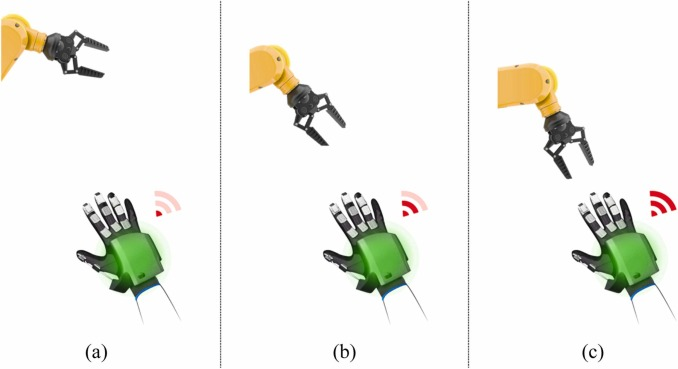
\includegraphics[width=0.9\linewidth]{figs/haptic-cues.jpg}
            \caption{Indicating the gripper’s destination using vibration on different human fingers.}
            \label{fig:sfig1}
        \end{subfigure}%
        \begin{subfigure}{.49\textwidth}
            \centering
            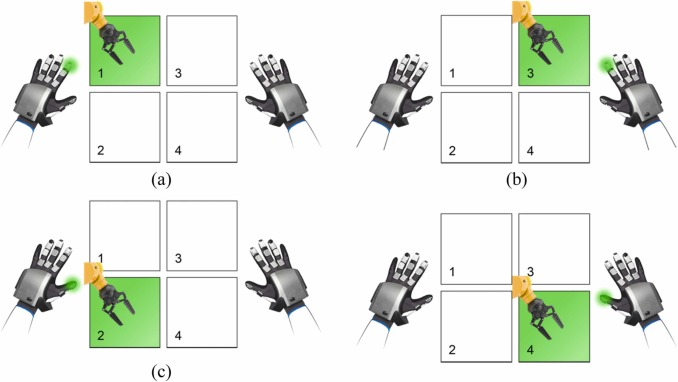
\includegraphics[width=0.9\linewidth]{figs/visual-cues.jpg}
            \caption{Indicating the proximity of gripper via change of vibration frequency.}
            \label{fig:sfig2}
        \end{subfigure}
        \caption{Visual and haptic interfaces used in the experiment \cite{CHU2023313}}
        \label{fig:haptic-visual-cues}
    \end{figure}

    \paragraph{\textbf{Experiment Design: Collaborative LEGO Assembly Task}}
    The experimental setup involved a human operator collaborating with a desktop robotic arm in a 25 cm × 25 cm workspace. The operator's task was to pick, fetch, and stack LEGO blocks onto specific areas of the workspace, sorted by color, while the robot arm delivered extra blocks randomly into the workspace over a wall. It aimed to verify and cross-compare the effectiveness of visual and haptic cues in conveying the robot’s intent to the human operator. Figures \ref{f:area-1} and \ref{f:robot-area-1} depict the collaborative workspace and robot setup.

    \begin{figure}[!htpb]
        \centering
        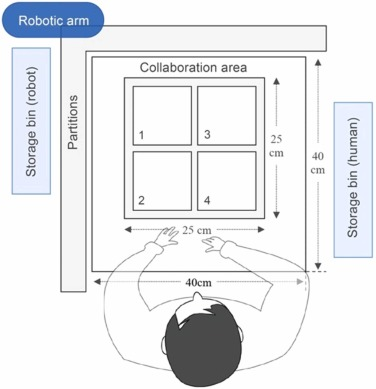
\includegraphics[width=0.4\linewidth]{figs/area-1.jpg}
        \caption{Collaborative work space in the experiment \cite{CHU2023313}}
        \label{f:area-1}
    \end{figure}

    \begin{figure}[!htpb]
        \centering
        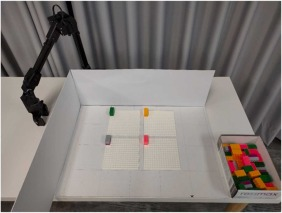
\includegraphics[width=0.4\linewidth]{figs/robot-area-1.jpg}
        \caption{Actual work environment in the experiment \cite{CHU2023313}}
        \label{f:robot-area-1}
    \end{figure}

    The operator and robot worked independently, without physical contact, adhering to a sequence of tasks. While the operator picked up blocks randomly and placed them in the correct colored area, the robot randomly delivered blocks from the storage bin to one of the four workspaces. This task required careful coordination to avoid collision and optimize assembly efficiency, highlighting the benefits of \ac{AR}-based interfaces.

    \paragraph{\textbf{System Framework}}
    UNITY engine running on a desktop computer allowed to communicat with the robot and the \ac{AR} devices. As shown in figure \ref{f:system-framework}, the system's architecture used USB connections and WiFi/Bluetooth for communication between the HoloLens, SenseGlove, and Robot. A HTC VIVE tracker was attached to the gloves to track the user's hand movements, providing haptic feedback in synchronization with the \ac{AR} visuals.

% remove this figure (done) - change the above text to reflect the removal of the figure
    % \begin{figure}[!htpb]
    %     \centering
    %     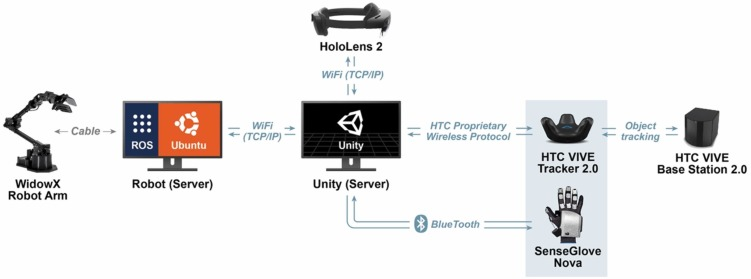
\includegraphics[width=0.75\linewidth]{figs/system-framework.jpg}
    %     \caption{The system framework for integration of hardware devices in the experiment \cite{CHU2023313}}
    %     \label{f:system-framework}
    % \end{figure}

    The framework allowed seamless interaction between the physical and virtual worlds, enabling real-time feedback for the operator, thus improving decision-making and task efficiency in the assembly process.

    \paragraph{\textbf{Advantages of Multimodal Cues}}
    The experiment demonstrated that using a combination of visual and haptic cues led to better task performance, as these cues helped the human operator predict the robot's movements, reduce visual strain, and enhance safety. The visual interfaces (especially those displaying proximity) outperformed others in usability, while haptic feedback was useful in environments where visual information might be insufficient or overloaded. Acoustic cues were also mentioned in the literature as a means to reduce anxiety in unpredictable robotic motions.

    % \paragraph{Conclusion}
    % The experiment with LEGO assembly and the integration of \ac{AR} and haptic feedback showed that visual and haptic \ac{AR} interfaces effectively communicate robot motion intent, improving interaction and collaboration. The system, using ROS and MoveIt, provided a flexible and scalable platform for HRC in a shared workspace. The findings of this study align well with current literature, which emphasizes the importance of multimodal feedback in enhancing human-robot interaction in smart manufacturing.

%  parece-me que a parte de cima parece estar bem estruturada e revelar as vantagens do artigo explorado - ver as referencias que faltam e organizar melhor a estrutura e as figuras - remover depois o texto comentado que está acima de toda esta parte que escrevi agora - 24 set 01h56

    %verificar este artigo e mencionar coisas mais úteis, isto está mto breve
    % Additionally, Lotsaris et al.~\cite{LOTSARIS2021301} presented an \ac{AR} application that facilitates operator work in human-robot environments by 
    % enabling coexistence and improving communication. Their system displays safety fields around the robot using different colors to represent safe and 
    % dangerous regions, enhancing situational awareness and reducing the risk of accidents. However, a significant challenge remains in the complexity of
    % recognizing detailed information through haptic feedback, indicating a need for more sophisticated algorithms and sensors to capture and translate 
    % complex robot actions into intuitive \ac{AR} visualizations.
    


%%%%%%%%%%%%%%%%%%%%%%%%%%%%% 24 set - 17h - deixar ??? ver o que este artigo diz e se é relevante
    % \item \textbf{Virtual and Augmented Reality for Intuitive Robot Programming}
    
    % Programming robots using Virtual Reality (VR) and \ac{DT} introduces innovative methods that capture human movements, reducing the learning curve for 
    % non-experts and enabling intuitive programming of complex tasks. Bolano et al.~\cite{Bolano2020} demonstrated that bilateral communication between 
    % the VR environment and the robot’s hardware allows changes to be made in both the virtual and physical systems. This full immersive experience 
    % enables users to interact directly with the robot's end effector through holographic interfaces, facilitating the selection and application of 
    % desired operations seamlessly.
    
    % Similarly, Burghardt et al.~\cite{burghardt2020programming} explored programming DTs using VR, where the robot reproduces human movements within a virtual 
    % environment. This approach ensures that the robot can accurately mimic complex human actions, which is particularly beneficial in tasks that are 
    % challenging to automate traditionally. The integration of Unity and \ac{ROS} platforms further enhances the functionality by 
    % providing robust communication and real-time data processing capabilities.
    
    % In the context of mobile platforms, Lotsaris et al.~\cite{LOTSARIS2021301} highlighted the challenges of achieving friendly interaction in shared 
    % working environments due to the absence of effective communication between operators and robots. Their AR application addresses this by displaying 
    % safety fields and facilitating better communication, thereby improving the overall interaction experience.
    
    % \begin{figure}[h]
    %     \centering
    %     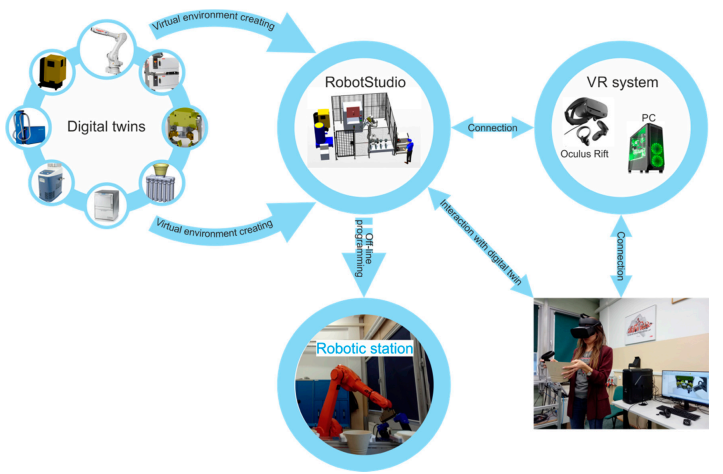
\includegraphics[width=0.9\linewidth]{figs/vr-oculos-dt.png}
    %     \caption{Schematic diagram of the building and programming of a robotic station alongside VR technologies \cite{burghardt2020programming}}
    %     \label{fig:vr-oculos-dt}
    % \end{figure}
    
    % Despite these advancements, challenges such as the need for high precision in replicating human movements and the complexity of \ac{VR} tracking 
    % technology persist. Improvements in algorithms, particularly those utilizing Machine Learning (\ac{ML}) techniques, are essential to ensure that 
    % robotic movements closely mimic human operators' actions \cite{Burghardt2020}.
    
    \item \textbf{AR-Assisted Multi-Robot Systems for Enhanced Control and Coordination}
    
    The use of \ac{AR} in real-time and planned control modes for multi-robot manufacturing systems significantly improves interaction, operational 
    safety, and efficiency. Li et al.~\cite{LI2022102321} demonstrated how operators can manage and coordinate multiple robots more effectively using 
    \ac{AR}-assisted DTs. Figure~\ref{fig:physical-digital} illustrates the dual view where users interact with the physical setup of two collaborating 
    robots and view their virtual counterparts via Microsoft Hololens \ac{AR} glasses. This immersive and intuitive control experience allows for 
    real-time simulation and monitoring of manufacturing processes and robot operations.
    
    \begin{figure}[!htpb]
        \centering
        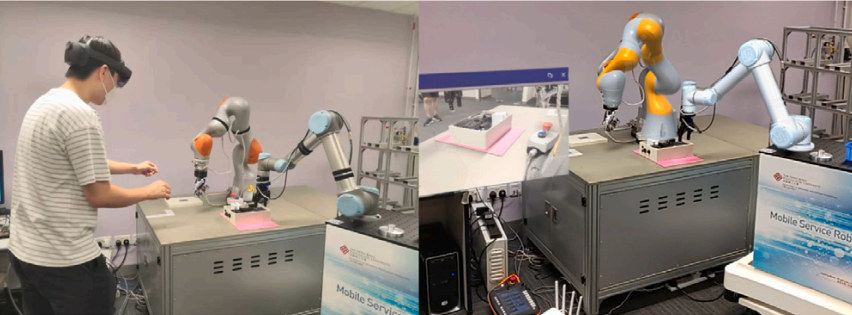
\includegraphics[width=0.85\linewidth]{figs/physical-digital.png}
        \caption{\ac{AR}-assisted \ac{DT}-enabled multi-robot collaborative manufacturing system \cite{LI2022102321}}
        \label{fig:physical-digital}
    \end{figure}

    Despite the promising advancements, issues such as \ac{DT} model accuracy and network latency continue to affect system performance. Future work must 
    focus on enhancing the fidelity and responsiveness of \ac{AR}-assisted \ac{DT} systems to fully realize their potential in industrial applications 
    \cite{LI2022102321}.

    Additionally, Ong et al.~\cite{ong2020} presented an AR-assisted robot programming system for welding applications. Their user-friendly interface 
    simplifies and accelerates the programming process by allowing users to define welding points and orientations using a handheld pointer. 
    The \ac{AR} interface enables users to validate programmed tasks within the real robot workspace, enhancing both accuracy and efficiency.
    
    Further advancements include the use of smart glasses and smartphones for robot manipulation. Malí et al.~\cite{7819154} developed an \ac{AR} 
    application that allows users to adjust robot axis values, highlight specific robot points with 3D arrows, navigate to invisible robot points using
    leading lines, and provide instructions via text and touch interactions. This system was evaluated in a production cell with an industrial robot, 
    demonstrating improved usability and interaction capabilities.

    Puljiz et al.~\cite{puljiz2019conceptsendtoendaugmentedreality,puljiz2} explored various AR-based methods for robotic arm programming using devices like Microsoft HoloLens. 
    Their approaches include hand-guided task programming, augmented trajectories, and the creation of spatial maps for waypoint placement and virtual 
    trajectory execution. These methods enable intuitive and precise programming of robotic arms, facilitating seamless integration of virtual instructions 
    with real-world robot operations.
    
    % analise do artigo - AR-assisted digital twin-enabled robot collaborative manufacturing system with human-in-the-loop - ref: LI2022102321
    In today's highly competitive market, manufacturing is evolving towards large-scale individualization and personalization, leading to an increased demand for flexibility and automation in manufacturing systems. To meet these personalization requirements, human operators are increasingly integrated into the production process~\cite{1}, collaborating with industrial robots that are well-developed and play a significant role in efficiently handling complex manufacturing tasks~\cite{2,3}.
    % rephrase this below sentence
    However, most existing robotic systems still carry out pre-programmed tasks in a routine manner with limited intelligence.

    To address this limitation, two effective human--robot collaborative alternatives have emerged. The first is robot learning, which aims to train robots by leveraging advanced \ac{AI} techniques~\cite{6}. The second, more pertinent to our interests, involves placing a human expert in-the-loop to teach or teleoperate the robot remotely.

    % reformulate this part
    % This second alternative represents the most useful approach, since it leverages the main concept of industry 5.0 (extend the existing capabilities of both humans and robots) - Integrating human intelligence in the multi-robot collaborative manufacturing process plays a promising role in today’s smart manufacturing to extend the existing capabilities of both humans and robots.
    
    Unlike traditional human--robot collaboration, multi-robot collaborative manufacturing with a human in the loop does not require workers to be physically present in the workspace or to collaborate solely in the physical realm. Instead, it enables manufacturing activities to be performed collaboratively with other equipment in a digitalized cyberspace by remotely teleoperating the robot. This paradigm is flexible in terms of space, safety, and technology, effectively bridging the gap between fully automated and fully manual manufacturing \cite{7}.

    
    Due to the complex scenario in manufacturing right now, there still exist several challenges to realize this human-in-the-loop collaborative manufacturing, such as:
    \begin{itemize}
        \item The lack of user-friendly interfaces for robot teleoperation, which require experienced operators to edit or program the robot.
        \item The need for a more intuitive and user-friendly robot teleoperation system that can be easily operated by operators with relevant experience in the manufacturing industry but lacking experience in robot operation \cite{9}.
    \end{itemize}

    % according to the related work:
    % Multi-agent based collaborative manufacturing:
    "The main research works in this field have focused on proposing technological solutions to improve safety, productivity, and reduce costs."
    In order to fill this research gap, wearable \ac{AR}-assisted system and \ac{DT} technologies allow users to observe and teleoperate the real robots accurately in an intuitive manner. 
    % onde por estas 2 partes?

    % AR-assisted robot teleoperation 
    In multi-agent-based collaborative manufacturing, research has primarily focused on technological solutions to enhance safety, increase productivity, and reduce costs. Robot teleoperation allows users to remotely operate robots manually without physical contact, using suitable interfaces like gamepads or keyboards. This control paradigm, benefiting from a close coupling between user input and robot actions, is widely studied in robot control. Owing to its temporal and spatial adaptability, robot teleoperation has been extensively applied in surgical robots~\cite{22}, robotic manipulators~\cite{11}, aerial robots~\cite{23}, and underwater robots~\cite{24}.
    %  confirm these citations above
    
    \ac{AR} enables workers to access both physical and virtual information in a hybrid environment and interact with virtual objects~\cite{26,27}. Thus, \ac{AR} is well-suited for teleoperation tasks, bridging the gap between human and machine systems \cite{this-article}. In recent years, various studies have combined \ac{AR} technology with robot teleoperation. For instance,~\cite{10} introduced an \ac{AR}-based teleoperation system utilizing RGB-D imaging and a posture demonstration device. This system transmits color and depth images of the remote robot environment to the local area, allowing the operator to perceive the environment and perform robot teleoperation.
    %  confirm these citations above
    
    Another example is an \ac{AR}-assisted robot programming system that transforms robot work scenes into \ac{AR} environments, facilitating fast and intuitive robot path planning and task programming \cite{30}.
    %  confirm these citations above

    \cite{32} utilized \ac{AR} to provide additional visual information about the environment and the robot, aiming to enhance the operator's visual field with cues, thereby improving task performance.
    %  confirm these citations above

    In smart manufacturing, recent studies have started to establish \ac{DT} of robots for device control purposes. For example, \cite{37} developed a \ac{DT} of a robot arm using the Unity engine to virtually learn manufacturing skills, which the physical robot arm could subsequently replicate in the physical space.
    %  confirm these citations above

    Recognizing that human involvement remains beneficial and necessary in certain cases,\cite{41} combined \acp{DT} and \ac{VR} interfaces to design an immersive human-in-the-loop robotic assembly system. Similarly, in\cite{42}, the \ac{DT} functioned as an intermediate layer between the operator and a controlled machine (e.g., a robot arm), facilitating interaction and monitoring the quality of remote tasks through an intuitive, low-latency interface.
    %  confirm these citations above

    Li et al ~\cite{this-article} proposed a framework for system design and implementation as an \ac{AR}-assisted, \ac{DT}-enabled robot collaborative manufacturing system featuring human-in-the-loop control.
    
    First, a multi-node communication mechanism is introduced to ensure effective communication among multiple robots and clients within the same system. Afterwards, the design of the \ac{AR}-based robot teleoperation system, including pose registration and motion planning, is detailed. Finally, three \ac{DT}-enabled interaction approaches are developed to achieve closed-loop interaction between the virtual and physical robots, resulting in an architecture described in the figure \ref{f:system-framework}.

    \begin{figure}[!htpb]
        \centering
        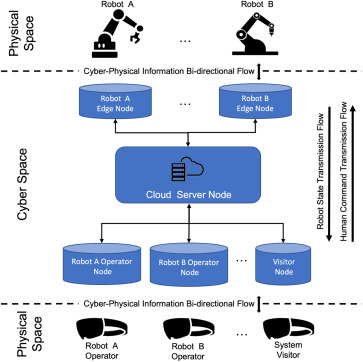
\includegraphics[width=0.5\linewidth]{figs/framework.jpg}
        \caption{The Architecture of Multi-robot Multi-client Communication Mechanism \cite{LI2022102321}}
        \label{f:system-framework}
    \end{figure}

    During information transmission, the control communication flow between each robot and client is encrypted using a hash table. Moreover, in manufacturing practice, the system utilizes commercial cloud servers and employs Secure Sockets Layer \ac{SSL} and \ac{SSTP} encryption methods to ensure system stability and security.

    To implement the concept of a multi-robot collaborative manufacturing system with human-in-the-loop control, a \ac{DT} of the physical robot is modeled using the Unity game engine. The robot twin is then ported to \ac{AR} glasses to enhance the immersive experience, providing both a teleoperation method and a more user-friendly observation approach for the robot. In the \ac{AR} glasses, the \ac{DT} of the robot, synchronized with the real robot, is projected as a hologram in the remote workspace. With the mapped \ac{DT} of the physical robot, remote control of the robot's movement is possible, while its state can be monitored and visualized via the robot \ac{DT}. By integrating the proposed communication mechanism and multiple \ac{AR} teleoperation systems, users can collaborate even when distributed across different locations, aligning with the collaborative manufacturing paradigm.

    The process of transferring the pose of the \ac{DT} to the physical robot, known as registration, consists mainly of two stages: displayed model alignment and joint alignment. In the model alignment stage, using the pre-designed virtual 3D robot model, the Vuforia Engine is employed to align the model targets between the physical and virtual robots, synchronizing the displayed robot pose. Joint value alignment then involves calculating a joint-value transformation matrix based on the pose-aligned models, converting the \ac{DT}'s joint values in the \ac{AR} coordinate system to the physical robot's joint values in the real-world coordinate system.


    Overall, a robot control method aided by \ac{AR} technology offers clear advantages over direct robot control, such as:
    \begin{itemize}
        \item Predictability for the final posture and motion trajectories of the physical robot.
        \item Visualization of trajectories to prevent potential safety issues.
        \item User-friendly interface, allowing the manufacturing system to be manipulated without spatial or human limitations.
    \end{itemize}

    Apart from controlling the robot, observing the environmental information of the workspace and the robot's state during task execution remains challenging. In the proposed system, IP cameras monitor the workspace, and the video feed is projected to the \ac{AR} glasses via a video streaming server. This setup allows both the status of the robot and the real-time status of the workspace to be presented in the \ac{AR} glasses, enhancing remote monitoring efficiency, as illustrated in figure \ref{f:workspace-visualization}.

    \begin{figure}[!htpb]
        \centering
        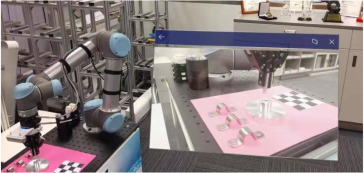
\includegraphics[width=0.7\linewidth]{figs/workspace-visualization.jpg}
        \caption{Demonstration of workspace observation approach \cite{LI2022102321}}
        \label{f:workspace-visualization}   
    \end{figure}
    \FloatBarrier

    Nevertheless, several challenges persist. Networking latency and positioning accuracy are issues presented in the lab-based demonstration. To address networking latency, some novel communication mechanisms (e.g., time-sensitive networks) and technologies (e.g., 5G) are proposed \cite{LI2022102321}. 


    % do a conclusion of the state of art. i will transition into the methodology of proposing the system - taking into consideration several aspects of the state of art such as: using Unity 3D for robot model development, trying to implement the billateral communication of digital twins by utilizing a robot that already has ROS working on it as well as the packages that allow it to move. besides that, the use of vuforia to do the pose registration of the robot. The suggestions of the visual and audio cues that can be implemented in AR.  the safety-zone interactions allow the user to be aware of the robot's movements and prevent accidents, as well as the audio implemented - these are great ideas.
    % the robot manipulation was implemented in an easy to understand by non-experient people, were implemented from the remote site - unity - by utilizing the Interface of an HHD device to manipulate each joint separately -  by pressing a publish button that will send the robot to the desired real location.
    %  from the ros side, by manipulating the robot through its console, unity digital twin will be updated in real time, and the robot position will be visible for the remote user by visualizing the robot's position in the HHD device.
    % the camera feed transmition is also good to mention because it allows the remote user to visualzie the workspace that is being worked on.

    % do a conclusion of the state of art.

\end{enumerate}

\section{Summary}

Even though significant advancements in \ac{MR}-\ac{DT} implementations over the past, the state-of-the-art literature predominantly focuses on developing applications for on-site personnel. Remote collaboration, particularly in human-robot interaction \ac{HRI} scenarios, has received comparatively less attention, highlighting the need for systems that effectively facilitate both on-site and remote collaboration.
% confirm if i can say this

Therefore, the proposed project aims to facilitate and integrate better remote collaboration by proposing a generalized conceptual system applicable across various application scenarios.

Despite having developed on-site features, such as digital twin pose registration alongside audio and visual cues, focus will be mainly on the remote collaboration part implementation and the billateral communication between users.

Unity 3D engine will be further explored for robot model development, \ac{ROS} will be used for robot control, and Vuforia for pose registration. It will also incorporate visual and audio cues to enhance user safety and awareness, \ac{MR} elements also implemented with Unity 3D. IP cameras will enable workspace monitoring. 

In conclusion, the proposed system will enable remote users to manipulate the robot using handheld devices, with the robot's real-time position displayed in the Unity digital twin. By addressing these challenges, the project aims to enhance remote collaboration in human-robot interaction scenarios, contributing to the broader field of \ac{MR}-\ac{DT} applications.


% %add this part somewhere
% from article: 9911168
% "AI, AR, DT and HRC approaches are employed in smart manufacturing to transform data processing into digital processing and controlling. 
% Therefore, designing smart systems will lead to high-quality real-time data exchange, zero wasted efforts and better data management [43]. 
% Focusing on HRC applications, HRC is the future alternative to conventional robotic and automation systems."

% %also add this part somewhere:
% from article: chang-ar-hrc
% " Augmented reality will only continue to mature into
% a more accessible technology, and its role in human–robot collaboration can become much
% more impactful and relevant to many different domains"





